\renewcommand{\theequation}{\theenumi}
\begin{enumerate}[label=\thesection.\arabic*.,ref=\thesection.\theenumi]
\numberwithin{equation}{enumi}
\item  Equal chords of a circle (or of congruent circles) subtend equal angles at the centre. 
\item  If the angles subtended by two chords of a circle (or of congruent circles) at the centre (corresponding centres) are equal, the chords are equal.
\item  The perpendicular from the centre of a circle to a chord bisects the chord. 
\item  The line drawn through the centre of a circle to bisect a chord is perpendicular to the chord.
\item  There is one and only one circle passing through three non-collinear points. 
\item  Equal chords of a circle (or of congruent circles) are equidistant from the centre (or corresponding centres).
\item Chords equidistant from the centre (or corresponding centres) of a circle (or of congruent circles) are equal.
\item  If two arcs of a circle are congruent, then their corresponding chords are equal and conversely if two chords of a circle are equal, then their corresponding arcs (minor, major) are congruent.
\item Congruent arcs of a circle subtend equal angles at the centre. 
\item  The angle subtended by an arc at the centre is double the angle subtended by it at any point on the remaining part of the circle.
\item Angles in the same segment of a circle are equal. \item  Angle in a semicircle is a right angle. 
\item  If a line segment joining two points subtends equal angles at two other points lying on the same side of the line containing the line segment, the four points lie on a circle. 
%\begin{enumerate}
%The  following Python code generates Fig. \ref{fig:tri_geo_8_tri_sss_py}
%
\begin{lstlisting}
codes/triangle.py
\end{lstlisting}
%\renewcommand{\theequation}{\theenumi}
%\begin{enumerate}[label=\thesection.\arabic*.,ref=\thesection.\theenumi]
%\numberwithin{equation}{enumi}
%\item The figure for the triangle obtained in the question looks like Fig. \ref{fig:tri_geo_8_tri_right_angle}.
%%with angles $\phase{ A},\phase{ C}$ and $\phase{ B}$ and sides $a, b$ and $c$.  The unique feature of this triangle is $\phase{ C}$ which is defined to be $90\degree$.
%with vertices A,B and C
%
%
%%\renewcommand{\thefigure}{\theenumi.\arabic{figure}}
%\begin{figure}[!ht]
%\centering
%\resizebox{\columnwidth}{!}{%\documentclass{standalone}
%
%\usepackage{tikz,pgf} %and any other packages or tikzlibraries your picture needs
%
%\begin{document}
%\resizebox{\columnwidth}{!}{
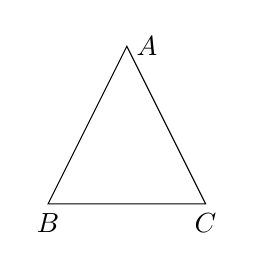
\begin{tikzpicture}
\draw (0,0) node[anchor=north]{$B$}
  -- (1,2) node[anchor=west]{$A$}
  -- (2,0) node[anchor=north]{$C$}
  -- cycle;
\end{tikzpicture}
%}
%\end{document}}
%\caption{Scalene Triangle by Latex-Tikz}
%\label{fig:tri_geo_8_tri_right_angle}	
%\end{figure}
%%
%%
%%\renewcommand{\thefigure}{\theenumi}
%%
%\item List the design parameters for construction
%\label{const:table1}
%\\
%\solution See Table. \ref{table:table1}. 
%%
%\begin{table}[ht!]
%\centering
%%\begin{tabular}{ |p{3cm}|p{3cm}|  }
%%\hline
%% \multicolumn{2}{|c|}{Initial Input Values.} \\
%%\hline
%%a & 4\\
%%\hline
%%b & 3\\
%%\hline
%%$\phase{(ACB)$ & $90^{\circ}$ \\
%%\hline
%%\end{tabular}
%%%%%%%%%%%%%%%%%%%%%%%%%%%%%%%%%%%%%%%%%%%%%%%%%%%%%%%%%%%%%%%%%%%%%%%
%%                                                                  %%
%%  This is the header of a LaTeX2e file exported from Gnumeric.    %%
%%                                                                  %%
%%  This file can be compiled as it stands or included in another   %%
%%  LaTeX document. The table is based on the longtable package so  %%
%%  the longtable options (headers, footers...) can be set in the   %%
%%  preamble section below (see PRAMBLE).                           %%
%%                                                                  %%
%%  To include the file in another, the following two lines must be %%
%%  in the including file:                                          %%
%%        \def\inputGnumericTable{}                                 %%
%%  at the beginning of the file and:                               %%
%%        \input{name-of-this-file.tex}                             %%
%%  where the table is to be placed. Note also that the including   %%
%%  file must use the following packages for the table to be        %%
%%  rendered correctly:                                             %%
%%    \usepackage[latin1]{inputenc}                                 %%
%%    \usepackage{color}                                            %%
%%    \usepackage{array}                                            %%
%%    \usepackage{longtable}                                        %%
%%    \usepackage{calc}                                             %%
%%    \usepackage{multirow}                                         %%
%%    \usepackage{hhline}                                           %%
%%    \usepackage{ifthen}                                           %%
%%  optionally (for landscape tables embedded in another document): %%
%%    \usepackage{lscape}                                           %%
%%                                                                  %%
%%%%%%%%%%%%%%%%%%%%%%%%%%%%%%%%%%%%%%%%%%%%%%%%%%%%%%%%%%%%%%%%%%%%%%



%%  This section checks if we are begin input into another file or  %%
%%  the file will be compiled alone. First use a macro taken from   %%
%%  the TeXbook ex 7.7 (suggestion of Han-Wen Nienhuys).            %%
\def\ifundefined#1{\expandafter\ifx\csname#1\endcsname\relax}


%%  Check for the \def token for inputed files. If it is not        %%
%%  defined, the file will be processed as a standalone and the     %%
%%  preamble will be used.                                          %%
\ifundefined{inputGnumericTable}

%%  We must be able to close or not the document at the end.        %%
	\def\gnumericTableEnd{\end{document}}


%%%%%%%%%%%%%%%%%%%%%%%%%%%%%%%%%%%%%%%%%%%%%%%%%%%%%%%%%%%%%%%%%%%%%%
%%                                                                  %%
%%  This is the PREAMBLE. Change these values to get the right      %%
%%  paper size and other niceties.                                  %%
%%                                                                  %%
%%%%%%%%%%%%%%%%%%%%%%%%%%%%%%%%%%%%%%%%%%%%%%%%%%%%%%%%%%%%%%%%%%%%%%

	\documentclass[12pt%
			  %,landscape%
                    ]{report}
       \usepackage[latin1]{inputenc}
       \usepackage{fullpage}
       \usepackage{color}
       \usepackage{array}
       \usepackage{longtable}
       \usepackage{calc}
       \usepackage{multirow}
       \usepackage{hhline}
       \usepackage{ifthen}
        \usepackage[cmex10]{amsmath}
       \newcommand{\myvec}[1]{\ensuremath{\begin{pmatrix}#1\end{pmatrix}}}

	\begin{document}


%%  End of the preamble for the standalone. The next section is for %%
%%  documents which are included into other LaTeX2e files.          %%
\else

%%  We are not a stand alone document. For a regular table, we will %%
%%  have no preamble and only define the closing to mean nothing.   %%
    \def\gnumericTableEnd{}

%%  If we want landscape mode in an embedded document, comment out  %%
%%  the line above and uncomment the two below. The table will      %%
%%  begin on a new page and run in landscape mode.                  %%
%       \def\gnumericTableEnd{\end{landscape}}
%       \begin{landscape}


%%  End of the else clause for this file being \input.              %%
\fi

%%%%%%%%%%%%%%%%%%%%%%%%%%%%%%%%%%%%%%%%%%%%%%%%%%%%%%%%%%%%%%%%%%%%%%
%%                                                                  %%
%%  The rest is the gnumeric table, except for the closing          %%
%%  statement. Changes below will alter the table's appearance.     %%
%%                                                                  %%
%%%%%%%%%%%%%%%%%%%%%%%%%%%%%%%%%%%%%%%%%%%%%%%%%%%%%%%%%%%%%%%%%%%%%%

\providecommand{\gnumericmathit}[1]{#1} 
%%  Uncomment the next line if you would like your numbers to be in %%
%%  italics if they are italizised in the gnumeric table.           %%
%\renewcommand{\gnumericmathit}[1]{\mathit{#1}}
\providecommand{\gnumericPB}[1]%
{\let\gnumericTemp=\\#1\let\\=\gnumericTemp\hspace{0pt}}
 \ifundefined{gnumericTableWidthDefined}
        \newlength{\gnumericTableWidth}
        \newlength{\gnumericTableWidthComplete}
        \newlength{\gnumericMultiRowLength}
        \global\def\gnumericTableWidthDefined{}
 \fi
%% The following setting protects this code from babel shorthands.  %%
 \ifthenelse{\isundefined{\languageshorthands}}{}{\languageshorthands{english}}
%%  The default table format retains the relative column widths of  %%
%%  gnumeric. They can easily be changed to c, r or l. In that case %%
%%  you may want to comment out the next line and uncomment the one %%
%%  thereafter                                                      %%
\providecommand\gnumbox{\makebox[0pt]}
%%\providecommand\gnumbox[1][]{\makebox}

%% to adjust positions in multirow situations                       %%
\setlength{\bigstrutjot}{\jot}
\setlength{\extrarowheight}{\doublerulesep}

%%  The \setlongtables command keeps column widths the same across  %%
%%  pages. Simply comment out next line for varying column widths.  %%
\setlongtables

\setlength\gnumericTableWidth{%
	71pt+%
	95pt+%
0pt}
\def\gumericNumCols{2}
\setlength\gnumericTableWidthComplete{\gnumericTableWidth+%
         \tabcolsep*\gumericNumCols*2+\arrayrulewidth*\gumericNumCols}
\ifthenelse{\lengthtest{\gnumericTableWidthComplete > \linewidth}}%
         {\def\gnumericScale{\ratio{\linewidth-%
                        \tabcolsep*\gumericNumCols*2-%
                        \arrayrulewidth*\gumericNumCols}%
{\gnumericTableWidth}}}%
{\def\gnumericScale{1}}

%%%%%%%%%%%%%%%%%%%%%%%%%%%%%%%%%%%%%%%%%%%%%%%%%%%%%%%%%%%%%%%%%%%%%%
%%                                                                  %%
%% The following are the widths of the various columns. We are      %%
%% defining them here because then they are easier to change.       %%
%% Depending on the cell formats we may use them more than once.    %%
%%                                                                  %%
%%%%%%%%%%%%%%%%%%%%%%%%%%%%%%%%%%%%%%%%%%%%%%%%%%%%%%%%%%%%%%%%%%%%%%

\ifthenelse{\isundefined{\gnumericColA}}{\newlength{\gnumericColA}}{}\settowidth{\gnumericColA}{\begin{tabular}{@{}p{71pt*\gnumericScale}@{}}x\end{tabular}}
\ifthenelse{\isundefined{\gnumericColB}}{\newlength{\gnumericColB}}{}\settowidth{\gnumericColB}{\begin{tabular}{@{}p{95pt*\gnumericScale}@{}}x\end{tabular}}

\begin{tabular}[c]{%
	b{\gnumericColA}%
	b{\gnumericColB}%
	}

%%%%%%%%%%%%%%%%%%%%%%%%%%%%%%%%%%%%%%%%%%%%%%%%%%%%%%%%%%%%%%%%%%%%%%
%%  The longtable options. (Caption, headers... see Goosens, p.124) %%
%	\caption{The Table Caption.}             \\	%
% \hline	% Across the top of the table.
%%  The rest of these options are table rows which are placed on    %%
%%  the first, last or every page. Use \multicolumn if you want.    %%

%%  Header for the first page.                                      %%
%	\multicolumn{2}{c}{The First Header} \\ \hline 
%	\multicolumn{1}{c}{colTag}	%Column 1
%	&\multicolumn{1}{c}{colTag}	\\ \hline %Last column
%	\endfirsthead

%%  The running header definition.                                  %%
%	\hline
%	\multicolumn{2}{l}{\ldots\small\slshape continued} \\ \hline
%	\multicolumn{1}{c}{colTag}	%Column 1
%	&\multicolumn{1}{c}{colTag}	\\ \hline %Last column
%	\endhead

%%  The running footer definition.                                  %%
%	\hline
%	\multicolumn{2}{r}{\small\slshape continued\ldots} \\
%	\endfoot

%%  The ending footer definition.                                   %%
%	\multicolumn{2}{c}{That's all folks} \\ \hline 
%	\endlastfoot
%%%%%%%%%%%%%%%%%%%%%%%%%%%%%%%%%%%%%%%%%%%%%%%%%%%%%%%%%%%%%%%%%%%%%%

\hhline{|--}
	 \multicolumn{2}{|p{	\gnumericColA+%
	\gnumericColB+%
	\tabcolsep*2*1}|}%
	{\gnumericPB{\centering}\gnumbox{Input values}}
\\
\hhline{|-|-|}
	 \multicolumn{1}{|p{\gnumericColA}|}%
	{\gnumericPB{\centering}\gnumbox{Parameters}}
	&\multicolumn{1}{p{\gnumericColB}|}%
	{\gnumericPB{\centering}\gnumbox{Values}}
\\
\hhline{|--|}
	 \multicolumn{1}{|p{\gnumericColA}|}%
	{\gnumericPB{\centering}\gnumbox{\textbf{O}}}
	&\multicolumn{1}{p{\gnumericColB}|}%
	{$\myvec{2\\-3}$}
\\
\hhline{|--|}
	 \multicolumn{1}{|p{\gnumericColA}|}%
	{\gnumericPB{\centering}\gnumbox{\textbf{A}}}
	&\multicolumn{1}{p{\gnumericColB}|}%
	{$\myvec{1\\4}$}
\\
\hhline{|-|-|}
\end{tabular}

\ifthenelse{\isundefined{\languageshorthands}}{}{\languageshorthands{\languagename}}
\gnumericTableEnd

%\caption{To construct $\triangle ABC$}
%\label{table:table1}	
%\end{table}
%
%%\item
%%	For simplicity, let the greek letter $\alpha = \phase{ B$.  We have the following definitions.
%%\begin{equation}
%%\label{eq:tri_trig_defs}
%%\begin{matrix}
%	%\sin \theta = \frac{b}{c} & 	\cos \theta = \frac{a}{c} \\
%	%\tan \theta = \frac{c}{a} & \cot \theta = \frac{1}{\tan \theta} \\
%	%\csc \theta = \frac{1}{\sin \theta} & \sec \theta = \frac{1}{\cos \theta}
%	%\end{equation}
%%
%\item Find the coordinates of the various points in Fig. \ref{fig:tri_geo_8_tri_right_angle}
%\label{const:tri_right_angle}
%\\
%
%\solution 
From the given information, 
%$\triangle ABC$ are 
\begin{align}
\label{eq:constr_a}
\vec{A} &= \myvec{4\\-6} 
\\
\vec{B} &= \myvec{3\\-2}, 
\label{eq:constr_b}
\\
\vec{C} &= \myvec{5\\2}
\label{eq:constr_c}
\end{align}
$\because \vec{M}$ is the midpoint of $AB$,
\begin{align}
\vec{M}= \frac{\vec{A}+\vec{B}}{2} = \frac{1}{2}\myvec{7\\-8}
\label{eq:constr_m}
\end{align}

$\because \vec{N}$ is the midpoint of $BC$,
\begin{align}
\vec{N}= \frac{\vec{B}+\vec{C}}{2} = \frac{1}{2}\myvec{8\\0}
\label{eq:constr_n}
\end{align}

$\because \vec{P}$ is the midpoint of $CA$,
\begin{align}
\vec{P}= \frac{\vec{C}+\vec{A}}{2} = \frac{1}{2}\myvec{9\\-4}
\label{eq:constr_p}
\end{align}
%
%Also, $\vec{M}$ is given to be the midpoint of $C$.  Hence, 
%\begin{align}
%\vec{M}&= \frac{\vec{C}+\vec{D}}{2}
%\\
%\implies \vec{D} &= 2 \vec{M} - \vec{C} = \myvec{a\\b}
%\label{eq:constr_d}
%\end{align}
%
%The values are listed in 
%%\item List the  derived values.
%%\label{const:table2}
%%\\
%%\solution See  
%Table. \ref{table:table2} 
%\begin{table}[ht!]
%\centering
%\begin{tabular}{ |p{3cm}|p{3cm}|  }
%\hline
% \multicolumn{2}{|c|}{Derived Values.} \\
%\hline
%$\vec{M}$ & $$\begin{pmatrix}3.5\\-4\end{pmatrix}$$\\						
%\hline
%$\vec{N}$ & $$\begin{pmatrix}4\\0\end{pmatrix} $$\\
%\hline
%$\vec{P}$ & $$\begin{pmatrix}4.5\\-2\end{pmatrix} $$\\
%\hline
%\end{tabular}
%\caption{To get Mid-points of $\triangle ABC$}
%\label{table:table2}
%\end{table}
%
%\item Draw Fig. \ref{fig:tri_geo_8_tri_right_angle}.	
%\\
%\solution 

The  following Python code verifies the determinant values.

\begin{lstlisting}
codes/determinant_check.py
\end{lstlisting}

\begin{figure}[!ht]
\centering
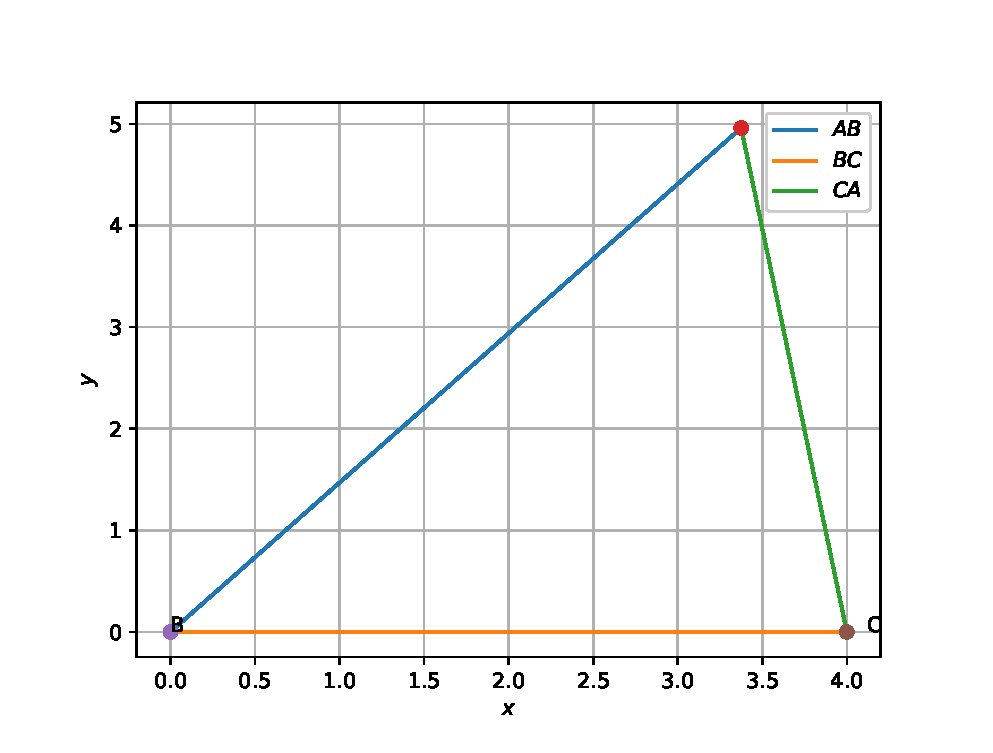
\includegraphics[width=\columnwidth]{./solutions/8/figs/triangle.eps}
\caption{Triangle generated using python}
\label{fig:tri_geo_8_tri_sss_py}
\end{figure}

%
%and the equivalent latex-tikz code generating Fig. \ref{fig:tri_geo_8_tri_right_angle} is 
%\begin{lstlisting}
%figs/triangle.tex
%\end{lstlisting}
%
%The above latex code can be compiled as a standalone document as
%\begin{lstlisting}
%figs/triangle_fig.tex
%\end{lstlisting}

%

%

%
%

%\end{enumerate}



%Let the balanced version of (\ref{eq:solutions/chem/6ato balance}) be
\begin{align}
    \label{eq:solutions/chem/6abalanced}x_{1}HNO_{3}+ x_{2}Ca(OH)_{2}\to x_{3}Ca(NO_{3})_{2}+ x_{4}H_{2}O
\end{align}

which results in the following equations:
\begin{align}
    (x_{1}+ 2x_{2}-2x_{4}) H= 0\\
    (x_{1}-2x_{3}) N= 0\\
    (3x_{1}+ 2x_{2}-6x_{3}- x_{4}) O=0\\
    (x_{2}-x_{3}) Ca= 0
\end{align}

which can be expressed as
\begin{align}
    x_{1}+ 2x_{2}+ 0.x_{3} -2x_{4} = 0\\
    x_{1}+ 0.x_{2} -2x_{3} +0.x_{4}= 0\\
    3x_{1}+ 2x_{2}-6x_{3}- x_{4} =0\\
    0.x_{1} +x_{2}-x_{3} +0.x_{4}= 0
\end{align}

resulting in the matrix equation
\begin{align}
    \label{eq:solutions/chem/6a matrix}
    \myvec{1 & 2 & 0 & -2\\
           1 & 0 & -2 & 0\\
           3 & 2 & -6 & -1\\
           0 & 1 & -1 & 0}\vec{x}
           =\vec{0}
\end{align}

where,
\begin{align}
   \vec{x}= \myvec{x_{1}\\x_{2}\\x_{3}\\x_{4}}
\end{align}

(\ref{eq:solutions/chem/6a matrix}) can be reduced as follows:
\begin{align}
    \myvec{1 & 2 & 0 & -2\\
           1 & 0 & -2 & 0\\
           3 & 2 & -6 & -1\\
           0 & 1 & -1 & 0}
    \xleftrightarrow[R_{3}\leftarrow \frac{R_3}{3}-R_{1}]{R_{2}\leftarrow R_2- R_1}
    \myvec{1 & 2 & 0 & -2\\
           0 & -2 & -2 & 2\\
           0 & -\frac{4}{3} & -2 & \frac{5}{3}\\
           0 & 1 & -1 & 0}\\
    \xleftrightarrow{R_2 \leftarrow -\frac{R_2}{2}}
    \myvec{1 & 2 & 0 & -2\\
          0 & 1 & 1 & -1\\
          0 & -\frac{4}{3} & -2 & \frac{5}{3}\\
          0 & 1 & -1 & 0}\\
    \xleftrightarrow[R_4 \leftarrow R_4- R_2]{R_3 \leftarrow R_3 + \frac{4}{3}R_2}
    \myvec{1 & 2 & 0 & -2\\
           0 & 1 & 1 & -1\\
           0 & 0 & -\frac{2}{3} & \frac{1}{3}\\
           0 & 0 & -2 & 1}\\
    \xleftrightarrow[R_3 \leftarrow -\frac{3}{2}R_3]{R_1 \leftarrow R_1- 2R_2}
    \myvec{1 & 0 & -2 & 0\\
           0 & 1 & 1 & -1\\
           0 & 0 & 1 & -\frac{1}{2}\\
           0 & 0 & -2 & 1}\\
    \xleftrightarrow{R_4\leftarrow R_4 + 2R_3}
    \myvec{1 & 0 & -2 & 0\\
           0 & 1 & 1 & -1\\
           0 & 0 & 1 & -\frac{1}{2}\\
           0 & 0 & 0 & 0}\\
    \xleftrightarrow[R_2\leftarrow R_2-R_3]{R_1\leftarrow R_1 + 2R_3}
    \myvec{1 & 0 & 0 & -1\\
           0 & 1 & 0 & -\frac{1}{2}\\
           0 & 0 & 1 & -\frac{1}{2}\\
           0 & 0 & 0 & 0}
\end{align}

Thus,
\begin{align}
    x_1=x_4, x_2= \frac{1}{2}x_4, x_3=\frac{1}{2}x_4\\
    \implies \quad\vec{x}= x_4\myvec{1\\ \frac{1}{2}\\ \frac{1}{2}\\1} =\myvec{2\\1\\1\\2}
\end{align} 
by substituting $x_4= 2$.

\hfill\break
%\vspace{5mm} 
Hence, (\ref{eq:solutions/chem/6abalanced}) finally becomes
\begin{align}
    2HNO_{3}+ Ca(OH)_{2}\to Ca(NO_{3})_{2}+ 2H_{2}O
\end{align}

%\end{enumerate}
\item  The sum of either pair of opposite angles of a cyclic quadrilateral is 180$\degree$.
\item  If sum of a pair of opposite angles of a quadrilateral is 180$\degree$, the quadrilateral is cyclic.
%
\item AB is a diameter of the circle, $CD$ is a chord equal to the radius of the circle. $AC$ and $BD$ when extended intersect at a point $E$. Prove that $\angle AEB = 60\degree$.
%\begin{enumerate}
%The  following Python code generates Fig. \ref{fig:tri_geo_8_tri_sss_py}
%
\begin{lstlisting}
codes/triangle.py
\end{lstlisting}
%\renewcommand{\theequation}{\theenumi}
%\begin{enumerate}[label=\thesection.\arabic*.,ref=\thesection.\theenumi]
%\numberwithin{equation}{enumi}
%\item The figure for the triangle obtained in the question looks like Fig. \ref{fig:tri_geo_8_tri_right_angle}.
%%with angles $\phase{ A},\phase{ C}$ and $\phase{ B}$ and sides $a, b$ and $c$.  The unique feature of this triangle is $\phase{ C}$ which is defined to be $90\degree$.
%with vertices A,B and C
%
%
%%\renewcommand{\thefigure}{\theenumi.\arabic{figure}}
%\begin{figure}[!ht]
%\centering
%\resizebox{\columnwidth}{!}{%\documentclass{standalone}
%
%\usepackage{tikz,pgf} %and any other packages or tikzlibraries your picture needs
%
%\begin{document}
%\resizebox{\columnwidth}{!}{
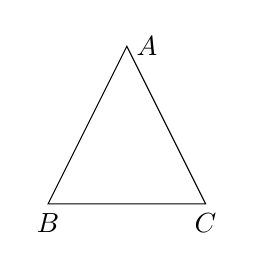
\begin{tikzpicture}
\draw (0,0) node[anchor=north]{$B$}
  -- (1,2) node[anchor=west]{$A$}
  -- (2,0) node[anchor=north]{$C$}
  -- cycle;
\end{tikzpicture}
%}
%\end{document}}
%\caption{Scalene Triangle by Latex-Tikz}
%\label{fig:tri_geo_8_tri_right_angle}	
%\end{figure}
%%
%%
%%\renewcommand{\thefigure}{\theenumi}
%%
%\item List the design parameters for construction
%\label{const:table1}
%\\
%\solution See Table. \ref{table:table1}. 
%%
%\begin{table}[ht!]
%\centering
%%\begin{tabular}{ |p{3cm}|p{3cm}|  }
%%\hline
%% \multicolumn{2}{|c|}{Initial Input Values.} \\
%%\hline
%%a & 4\\
%%\hline
%%b & 3\\
%%\hline
%%$\phase{(ACB)$ & $90^{\circ}$ \\
%%\hline
%%\end{tabular}
%%%%%%%%%%%%%%%%%%%%%%%%%%%%%%%%%%%%%%%%%%%%%%%%%%%%%%%%%%%%%%%%%%%%%%%
%%                                                                  %%
%%  This is the header of a LaTeX2e file exported from Gnumeric.    %%
%%                                                                  %%
%%  This file can be compiled as it stands or included in another   %%
%%  LaTeX document. The table is based on the longtable package so  %%
%%  the longtable options (headers, footers...) can be set in the   %%
%%  preamble section below (see PRAMBLE).                           %%
%%                                                                  %%
%%  To include the file in another, the following two lines must be %%
%%  in the including file:                                          %%
%%        \def\inputGnumericTable{}                                 %%
%%  at the beginning of the file and:                               %%
%%        \input{name-of-this-file.tex}                             %%
%%  where the table is to be placed. Note also that the including   %%
%%  file must use the following packages for the table to be        %%
%%  rendered correctly:                                             %%
%%    \usepackage[latin1]{inputenc}                                 %%
%%    \usepackage{color}                                            %%
%%    \usepackage{array}                                            %%
%%    \usepackage{longtable}                                        %%
%%    \usepackage{calc}                                             %%
%%    \usepackage{multirow}                                         %%
%%    \usepackage{hhline}                                           %%
%%    \usepackage{ifthen}                                           %%
%%  optionally (for landscape tables embedded in another document): %%
%%    \usepackage{lscape}                                           %%
%%                                                                  %%
%%%%%%%%%%%%%%%%%%%%%%%%%%%%%%%%%%%%%%%%%%%%%%%%%%%%%%%%%%%%%%%%%%%%%%



%%  This section checks if we are begin input into another file or  %%
%%  the file will be compiled alone. First use a macro taken from   %%
%%  the TeXbook ex 7.7 (suggestion of Han-Wen Nienhuys).            %%
\def\ifundefined#1{\expandafter\ifx\csname#1\endcsname\relax}


%%  Check for the \def token for inputed files. If it is not        %%
%%  defined, the file will be processed as a standalone and the     %%
%%  preamble will be used.                                          %%
\ifundefined{inputGnumericTable}

%%  We must be able to close or not the document at the end.        %%
	\def\gnumericTableEnd{\end{document}}


%%%%%%%%%%%%%%%%%%%%%%%%%%%%%%%%%%%%%%%%%%%%%%%%%%%%%%%%%%%%%%%%%%%%%%
%%                                                                  %%
%%  This is the PREAMBLE. Change these values to get the right      %%
%%  paper size and other niceties.                                  %%
%%                                                                  %%
%%%%%%%%%%%%%%%%%%%%%%%%%%%%%%%%%%%%%%%%%%%%%%%%%%%%%%%%%%%%%%%%%%%%%%

	\documentclass[12pt%
			  %,landscape%
                    ]{report}
       \usepackage[latin1]{inputenc}
       \usepackage{fullpage}
       \usepackage{color}
       \usepackage{array}
       \usepackage{longtable}
       \usepackage{calc}
       \usepackage{multirow}
       \usepackage{hhline}
       \usepackage{ifthen}
        \usepackage[cmex10]{amsmath}
       \newcommand{\myvec}[1]{\ensuremath{\begin{pmatrix}#1\end{pmatrix}}}

	\begin{document}


%%  End of the preamble for the standalone. The next section is for %%
%%  documents which are included into other LaTeX2e files.          %%
\else

%%  We are not a stand alone document. For a regular table, we will %%
%%  have no preamble and only define the closing to mean nothing.   %%
    \def\gnumericTableEnd{}

%%  If we want landscape mode in an embedded document, comment out  %%
%%  the line above and uncomment the two below. The table will      %%
%%  begin on a new page and run in landscape mode.                  %%
%       \def\gnumericTableEnd{\end{landscape}}
%       \begin{landscape}


%%  End of the else clause for this file being \input.              %%
\fi

%%%%%%%%%%%%%%%%%%%%%%%%%%%%%%%%%%%%%%%%%%%%%%%%%%%%%%%%%%%%%%%%%%%%%%
%%                                                                  %%
%%  The rest is the gnumeric table, except for the closing          %%
%%  statement. Changes below will alter the table's appearance.     %%
%%                                                                  %%
%%%%%%%%%%%%%%%%%%%%%%%%%%%%%%%%%%%%%%%%%%%%%%%%%%%%%%%%%%%%%%%%%%%%%%

\providecommand{\gnumericmathit}[1]{#1} 
%%  Uncomment the next line if you would like your numbers to be in %%
%%  italics if they are italizised in the gnumeric table.           %%
%\renewcommand{\gnumericmathit}[1]{\mathit{#1}}
\providecommand{\gnumericPB}[1]%
{\let\gnumericTemp=\\#1\let\\=\gnumericTemp\hspace{0pt}}
 \ifundefined{gnumericTableWidthDefined}
        \newlength{\gnumericTableWidth}
        \newlength{\gnumericTableWidthComplete}
        \newlength{\gnumericMultiRowLength}
        \global\def\gnumericTableWidthDefined{}
 \fi
%% The following setting protects this code from babel shorthands.  %%
 \ifthenelse{\isundefined{\languageshorthands}}{}{\languageshorthands{english}}
%%  The default table format retains the relative column widths of  %%
%%  gnumeric. They can easily be changed to c, r or l. In that case %%
%%  you may want to comment out the next line and uncomment the one %%
%%  thereafter                                                      %%
\providecommand\gnumbox{\makebox[0pt]}
%%\providecommand\gnumbox[1][]{\makebox}

%% to adjust positions in multirow situations                       %%
\setlength{\bigstrutjot}{\jot}
\setlength{\extrarowheight}{\doublerulesep}

%%  The \setlongtables command keeps column widths the same across  %%
%%  pages. Simply comment out next line for varying column widths.  %%
\setlongtables

\setlength\gnumericTableWidth{%
	71pt+%
	95pt+%
0pt}
\def\gumericNumCols{2}
\setlength\gnumericTableWidthComplete{\gnumericTableWidth+%
         \tabcolsep*\gumericNumCols*2+\arrayrulewidth*\gumericNumCols}
\ifthenelse{\lengthtest{\gnumericTableWidthComplete > \linewidth}}%
         {\def\gnumericScale{\ratio{\linewidth-%
                        \tabcolsep*\gumericNumCols*2-%
                        \arrayrulewidth*\gumericNumCols}%
{\gnumericTableWidth}}}%
{\def\gnumericScale{1}}

%%%%%%%%%%%%%%%%%%%%%%%%%%%%%%%%%%%%%%%%%%%%%%%%%%%%%%%%%%%%%%%%%%%%%%
%%                                                                  %%
%% The following are the widths of the various columns. We are      %%
%% defining them here because then they are easier to change.       %%
%% Depending on the cell formats we may use them more than once.    %%
%%                                                                  %%
%%%%%%%%%%%%%%%%%%%%%%%%%%%%%%%%%%%%%%%%%%%%%%%%%%%%%%%%%%%%%%%%%%%%%%

\ifthenelse{\isundefined{\gnumericColA}}{\newlength{\gnumericColA}}{}\settowidth{\gnumericColA}{\begin{tabular}{@{}p{71pt*\gnumericScale}@{}}x\end{tabular}}
\ifthenelse{\isundefined{\gnumericColB}}{\newlength{\gnumericColB}}{}\settowidth{\gnumericColB}{\begin{tabular}{@{}p{95pt*\gnumericScale}@{}}x\end{tabular}}

\begin{tabular}[c]{%
	b{\gnumericColA}%
	b{\gnumericColB}%
	}

%%%%%%%%%%%%%%%%%%%%%%%%%%%%%%%%%%%%%%%%%%%%%%%%%%%%%%%%%%%%%%%%%%%%%%
%%  The longtable options. (Caption, headers... see Goosens, p.124) %%
%	\caption{The Table Caption.}             \\	%
% \hline	% Across the top of the table.
%%  The rest of these options are table rows which are placed on    %%
%%  the first, last or every page. Use \multicolumn if you want.    %%

%%  Header for the first page.                                      %%
%	\multicolumn{2}{c}{The First Header} \\ \hline 
%	\multicolumn{1}{c}{colTag}	%Column 1
%	&\multicolumn{1}{c}{colTag}	\\ \hline %Last column
%	\endfirsthead

%%  The running header definition.                                  %%
%	\hline
%	\multicolumn{2}{l}{\ldots\small\slshape continued} \\ \hline
%	\multicolumn{1}{c}{colTag}	%Column 1
%	&\multicolumn{1}{c}{colTag}	\\ \hline %Last column
%	\endhead

%%  The running footer definition.                                  %%
%	\hline
%	\multicolumn{2}{r}{\small\slshape continued\ldots} \\
%	\endfoot

%%  The ending footer definition.                                   %%
%	\multicolumn{2}{c}{That's all folks} \\ \hline 
%	\endlastfoot
%%%%%%%%%%%%%%%%%%%%%%%%%%%%%%%%%%%%%%%%%%%%%%%%%%%%%%%%%%%%%%%%%%%%%%

\hhline{|--}
	 \multicolumn{2}{|p{	\gnumericColA+%
	\gnumericColB+%
	\tabcolsep*2*1}|}%
	{\gnumericPB{\centering}\gnumbox{Input values}}
\\
\hhline{|-|-|}
	 \multicolumn{1}{|p{\gnumericColA}|}%
	{\gnumericPB{\centering}\gnumbox{Parameters}}
	&\multicolumn{1}{p{\gnumericColB}|}%
	{\gnumericPB{\centering}\gnumbox{Values}}
\\
\hhline{|--|}
	 \multicolumn{1}{|p{\gnumericColA}|}%
	{\gnumericPB{\centering}\gnumbox{\textbf{O}}}
	&\multicolumn{1}{p{\gnumericColB}|}%
	{$\myvec{2\\-3}$}
\\
\hhline{|--|}
	 \multicolumn{1}{|p{\gnumericColA}|}%
	{\gnumericPB{\centering}\gnumbox{\textbf{A}}}
	&\multicolumn{1}{p{\gnumericColB}|}%
	{$\myvec{1\\4}$}
\\
\hhline{|-|-|}
\end{tabular}

\ifthenelse{\isundefined{\languageshorthands}}{}{\languageshorthands{\languagename}}
\gnumericTableEnd

%\caption{To construct $\triangle ABC$}
%\label{table:table1}	
%\end{table}
%
%%\item
%%	For simplicity, let the greek letter $\alpha = \phase{ B$.  We have the following definitions.
%%\begin{equation}
%%\label{eq:tri_trig_defs}
%%\begin{matrix}
%	%\sin \theta = \frac{b}{c} & 	\cos \theta = \frac{a}{c} \\
%	%\tan \theta = \frac{c}{a} & \cot \theta = \frac{1}{\tan \theta} \\
%	%\csc \theta = \frac{1}{\sin \theta} & \sec \theta = \frac{1}{\cos \theta}
%	%\end{equation}
%%
%\item Find the coordinates of the various points in Fig. \ref{fig:tri_geo_8_tri_right_angle}
%\label{const:tri_right_angle}
%\\
%
%\solution 
From the given information, 
%$\triangle ABC$ are 
\begin{align}
\label{eq:constr_a}
\vec{A} &= \myvec{4\\-6} 
\\
\vec{B} &= \myvec{3\\-2}, 
\label{eq:constr_b}
\\
\vec{C} &= \myvec{5\\2}
\label{eq:constr_c}
\end{align}
$\because \vec{M}$ is the midpoint of $AB$,
\begin{align}
\vec{M}= \frac{\vec{A}+\vec{B}}{2} = \frac{1}{2}\myvec{7\\-8}
\label{eq:constr_m}
\end{align}

$\because \vec{N}$ is the midpoint of $BC$,
\begin{align}
\vec{N}= \frac{\vec{B}+\vec{C}}{2} = \frac{1}{2}\myvec{8\\0}
\label{eq:constr_n}
\end{align}

$\because \vec{P}$ is the midpoint of $CA$,
\begin{align}
\vec{P}= \frac{\vec{C}+\vec{A}}{2} = \frac{1}{2}\myvec{9\\-4}
\label{eq:constr_p}
\end{align}
%
%Also, $\vec{M}$ is given to be the midpoint of $C$.  Hence, 
%\begin{align}
%\vec{M}&= \frac{\vec{C}+\vec{D}}{2}
%\\
%\implies \vec{D} &= 2 \vec{M} - \vec{C} = \myvec{a\\b}
%\label{eq:constr_d}
%\end{align}
%
%The values are listed in 
%%\item List the  derived values.
%%\label{const:table2}
%%\\
%%\solution See  
%Table. \ref{table:table2} 
%\begin{table}[ht!]
%\centering
%\begin{tabular}{ |p{3cm}|p{3cm}|  }
%\hline
% \multicolumn{2}{|c|}{Derived Values.} \\
%\hline
%$\vec{M}$ & $$\begin{pmatrix}3.5\\-4\end{pmatrix}$$\\						
%\hline
%$\vec{N}$ & $$\begin{pmatrix}4\\0\end{pmatrix} $$\\
%\hline
%$\vec{P}$ & $$\begin{pmatrix}4.5\\-2\end{pmatrix} $$\\
%\hline
%\end{tabular}
%\caption{To get Mid-points of $\triangle ABC$}
%\label{table:table2}
%\end{table}
%
%\item Draw Fig. \ref{fig:tri_geo_8_tri_right_angle}.	
%\\
%\solution 

The  following Python code verifies the determinant values.

\begin{lstlisting}
codes/determinant_check.py
\end{lstlisting}

\begin{figure}[!ht]
\centering
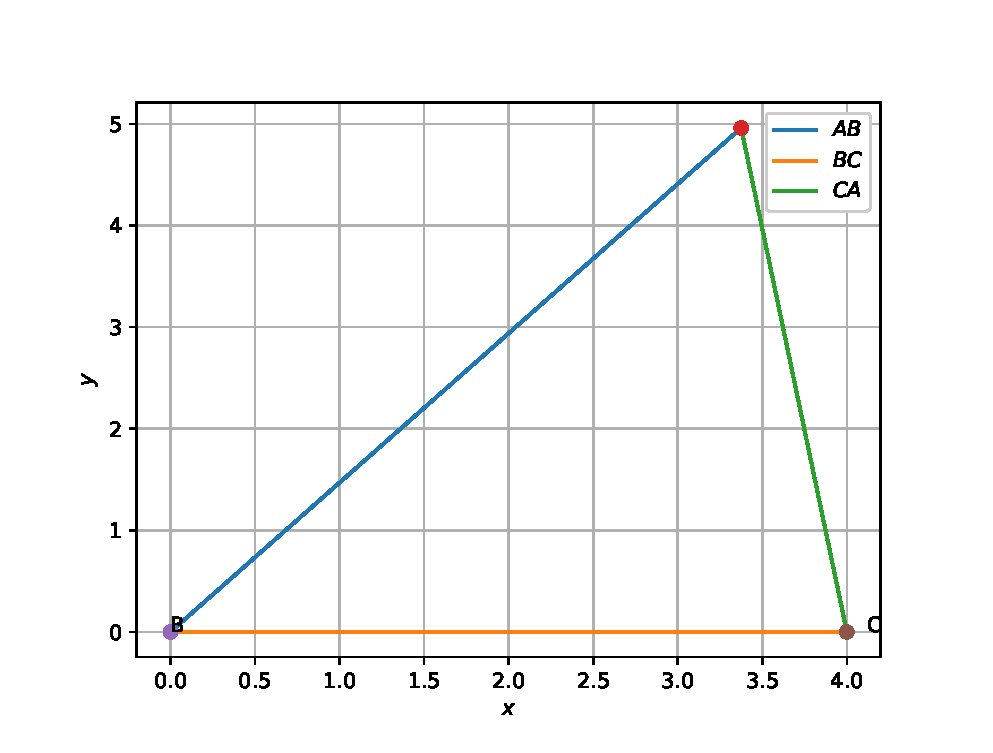
\includegraphics[width=\columnwidth]{./solutions/8/figs/triangle.eps}
\caption{Triangle generated using python}
\label{fig:tri_geo_8_tri_sss_py}
\end{figure}

%
%and the equivalent latex-tikz code generating Fig. \ref{fig:tri_geo_8_tri_right_angle} is 
%\begin{lstlisting}
%figs/triangle.tex
%\end{lstlisting}
%
%The above latex code can be compiled as a standalone document as
%\begin{lstlisting}
%figs/triangle_fig.tex
%\end{lstlisting}

%

%

%
%

%\end{enumerate}



%Let the balanced version of (\ref{eq:solutions/chem/6ato balance}) be
\begin{align}
    \label{eq:solutions/chem/6abalanced}x_{1}HNO_{3}+ x_{2}Ca(OH)_{2}\to x_{3}Ca(NO_{3})_{2}+ x_{4}H_{2}O
\end{align}

which results in the following equations:
\begin{align}
    (x_{1}+ 2x_{2}-2x_{4}) H= 0\\
    (x_{1}-2x_{3}) N= 0\\
    (3x_{1}+ 2x_{2}-6x_{3}- x_{4}) O=0\\
    (x_{2}-x_{3}) Ca= 0
\end{align}

which can be expressed as
\begin{align}
    x_{1}+ 2x_{2}+ 0.x_{3} -2x_{4} = 0\\
    x_{1}+ 0.x_{2} -2x_{3} +0.x_{4}= 0\\
    3x_{1}+ 2x_{2}-6x_{3}- x_{4} =0\\
    0.x_{1} +x_{2}-x_{3} +0.x_{4}= 0
\end{align}

resulting in the matrix equation
\begin{align}
    \label{eq:solutions/chem/6a matrix}
    \myvec{1 & 2 & 0 & -2\\
           1 & 0 & -2 & 0\\
           3 & 2 & -6 & -1\\
           0 & 1 & -1 & 0}\vec{x}
           =\vec{0}
\end{align}

where,
\begin{align}
   \vec{x}= \myvec{x_{1}\\x_{2}\\x_{3}\\x_{4}}
\end{align}

(\ref{eq:solutions/chem/6a matrix}) can be reduced as follows:
\begin{align}
    \myvec{1 & 2 & 0 & -2\\
           1 & 0 & -2 & 0\\
           3 & 2 & -6 & -1\\
           0 & 1 & -1 & 0}
    \xleftrightarrow[R_{3}\leftarrow \frac{R_3}{3}-R_{1}]{R_{2}\leftarrow R_2- R_1}
    \myvec{1 & 2 & 0 & -2\\
           0 & -2 & -2 & 2\\
           0 & -\frac{4}{3} & -2 & \frac{5}{3}\\
           0 & 1 & -1 & 0}\\
    \xleftrightarrow{R_2 \leftarrow -\frac{R_2}{2}}
    \myvec{1 & 2 & 0 & -2\\
          0 & 1 & 1 & -1\\
          0 & -\frac{4}{3} & -2 & \frac{5}{3}\\
          0 & 1 & -1 & 0}\\
    \xleftrightarrow[R_4 \leftarrow R_4- R_2]{R_3 \leftarrow R_3 + \frac{4}{3}R_2}
    \myvec{1 & 2 & 0 & -2\\
           0 & 1 & 1 & -1\\
           0 & 0 & -\frac{2}{3} & \frac{1}{3}\\
           0 & 0 & -2 & 1}\\
    \xleftrightarrow[R_3 \leftarrow -\frac{3}{2}R_3]{R_1 \leftarrow R_1- 2R_2}
    \myvec{1 & 0 & -2 & 0\\
           0 & 1 & 1 & -1\\
           0 & 0 & 1 & -\frac{1}{2}\\
           0 & 0 & -2 & 1}\\
    \xleftrightarrow{R_4\leftarrow R_4 + 2R_3}
    \myvec{1 & 0 & -2 & 0\\
           0 & 1 & 1 & -1\\
           0 & 0 & 1 & -\frac{1}{2}\\
           0 & 0 & 0 & 0}\\
    \xleftrightarrow[R_2\leftarrow R_2-R_3]{R_1\leftarrow R_1 + 2R_3}
    \myvec{1 & 0 & 0 & -1\\
           0 & 1 & 0 & -\frac{1}{2}\\
           0 & 0 & 1 & -\frac{1}{2}\\
           0 & 0 & 0 & 0}
\end{align}

Thus,
\begin{align}
    x_1=x_4, x_2= \frac{1}{2}x_4, x_3=\frac{1}{2}x_4\\
    \implies \quad\vec{x}= x_4\myvec{1\\ \frac{1}{2}\\ \frac{1}{2}\\1} =\myvec{2\\1\\1\\2}
\end{align} 
by substituting $x_4= 2$.

\hfill\break
%\vspace{5mm} 
Hence, (\ref{eq:solutions/chem/6abalanced}) finally becomes
\begin{align}
    2HNO_{3}+ Ca(OH)_{2}\to Ca(NO_{3})_{2}+ 2H_{2}O
\end{align}

%\end{enumerate}

\item $ABCD$ is a cyclic quadrilateral in which $AC$ and $BD$ are its diagonals. If $\angle DBC = 55\degree$ and $\angle BAC = 45\degree$, find $\angle BCD$
\item Two circles intersect at two points $A and B$. $AD$ and $AC$ are diameters to the two circles. Prove that $B$ lies on the line segment $DC$.
\item Prove that the quadrilateral formed (if possible) by the internal angle bisectors of any quadrilateral is cyclic.
%\begin{enumerate}
%The  following Python code generates Fig. \ref{fig:tri_geo_8_tri_sss_py}
%
\begin{lstlisting}
codes/triangle.py
\end{lstlisting}
%\renewcommand{\theequation}{\theenumi}
%\begin{enumerate}[label=\thesection.\arabic*.,ref=\thesection.\theenumi]
%\numberwithin{equation}{enumi}
%\item The figure for the triangle obtained in the question looks like Fig. \ref{fig:tri_geo_8_tri_right_angle}.
%%with angles $\phase{ A},\phase{ C}$ and $\phase{ B}$ and sides $a, b$ and $c$.  The unique feature of this triangle is $\phase{ C}$ which is defined to be $90\degree$.
%with vertices A,B and C
%
%
%%\renewcommand{\thefigure}{\theenumi.\arabic{figure}}
%\begin{figure}[!ht]
%\centering
%\resizebox{\columnwidth}{!}{%\documentclass{standalone}
%
%\usepackage{tikz,pgf} %and any other packages or tikzlibraries your picture needs
%
%\begin{document}
%\resizebox{\columnwidth}{!}{
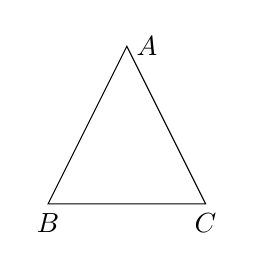
\begin{tikzpicture}
\draw (0,0) node[anchor=north]{$B$}
  -- (1,2) node[anchor=west]{$A$}
  -- (2,0) node[anchor=north]{$C$}
  -- cycle;
\end{tikzpicture}
%}
%\end{document}}
%\caption{Scalene Triangle by Latex-Tikz}
%\label{fig:tri_geo_8_tri_right_angle}	
%\end{figure}
%%
%%
%%\renewcommand{\thefigure}{\theenumi}
%%
%\item List the design parameters for construction
%\label{const:table1}
%\\
%\solution See Table. \ref{table:table1}. 
%%
%\begin{table}[ht!]
%\centering
%%\begin{tabular}{ |p{3cm}|p{3cm}|  }
%%\hline
%% \multicolumn{2}{|c|}{Initial Input Values.} \\
%%\hline
%%a & 4\\
%%\hline
%%b & 3\\
%%\hline
%%$\phase{(ACB)$ & $90^{\circ}$ \\
%%\hline
%%\end{tabular}
%%%%%%%%%%%%%%%%%%%%%%%%%%%%%%%%%%%%%%%%%%%%%%%%%%%%%%%%%%%%%%%%%%%%%%%
%%                                                                  %%
%%  This is the header of a LaTeX2e file exported from Gnumeric.    %%
%%                                                                  %%
%%  This file can be compiled as it stands or included in another   %%
%%  LaTeX document. The table is based on the longtable package so  %%
%%  the longtable options (headers, footers...) can be set in the   %%
%%  preamble section below (see PRAMBLE).                           %%
%%                                                                  %%
%%  To include the file in another, the following two lines must be %%
%%  in the including file:                                          %%
%%        \def\inputGnumericTable{}                                 %%
%%  at the beginning of the file and:                               %%
%%        \input{name-of-this-file.tex}                             %%
%%  where the table is to be placed. Note also that the including   %%
%%  file must use the following packages for the table to be        %%
%%  rendered correctly:                                             %%
%%    \usepackage[latin1]{inputenc}                                 %%
%%    \usepackage{color}                                            %%
%%    \usepackage{array}                                            %%
%%    \usepackage{longtable}                                        %%
%%    \usepackage{calc}                                             %%
%%    \usepackage{multirow}                                         %%
%%    \usepackage{hhline}                                           %%
%%    \usepackage{ifthen}                                           %%
%%  optionally (for landscape tables embedded in another document): %%
%%    \usepackage{lscape}                                           %%
%%                                                                  %%
%%%%%%%%%%%%%%%%%%%%%%%%%%%%%%%%%%%%%%%%%%%%%%%%%%%%%%%%%%%%%%%%%%%%%%



%%  This section checks if we are begin input into another file or  %%
%%  the file will be compiled alone. First use a macro taken from   %%
%%  the TeXbook ex 7.7 (suggestion of Han-Wen Nienhuys).            %%
\def\ifundefined#1{\expandafter\ifx\csname#1\endcsname\relax}


%%  Check for the \def token for inputed files. If it is not        %%
%%  defined, the file will be processed as a standalone and the     %%
%%  preamble will be used.                                          %%
\ifundefined{inputGnumericTable}

%%  We must be able to close or not the document at the end.        %%
	\def\gnumericTableEnd{\end{document}}


%%%%%%%%%%%%%%%%%%%%%%%%%%%%%%%%%%%%%%%%%%%%%%%%%%%%%%%%%%%%%%%%%%%%%%
%%                                                                  %%
%%  This is the PREAMBLE. Change these values to get the right      %%
%%  paper size and other niceties.                                  %%
%%                                                                  %%
%%%%%%%%%%%%%%%%%%%%%%%%%%%%%%%%%%%%%%%%%%%%%%%%%%%%%%%%%%%%%%%%%%%%%%

	\documentclass[12pt%
			  %,landscape%
                    ]{report}
       \usepackage[latin1]{inputenc}
       \usepackage{fullpage}
       \usepackage{color}
       \usepackage{array}
       \usepackage{longtable}
       \usepackage{calc}
       \usepackage{multirow}
       \usepackage{hhline}
       \usepackage{ifthen}
        \usepackage[cmex10]{amsmath}
       \newcommand{\myvec}[1]{\ensuremath{\begin{pmatrix}#1\end{pmatrix}}}

	\begin{document}


%%  End of the preamble for the standalone. The next section is for %%
%%  documents which are included into other LaTeX2e files.          %%
\else

%%  We are not a stand alone document. For a regular table, we will %%
%%  have no preamble and only define the closing to mean nothing.   %%
    \def\gnumericTableEnd{}

%%  If we want landscape mode in an embedded document, comment out  %%
%%  the line above and uncomment the two below. The table will      %%
%%  begin on a new page and run in landscape mode.                  %%
%       \def\gnumericTableEnd{\end{landscape}}
%       \begin{landscape}


%%  End of the else clause for this file being \input.              %%
\fi

%%%%%%%%%%%%%%%%%%%%%%%%%%%%%%%%%%%%%%%%%%%%%%%%%%%%%%%%%%%%%%%%%%%%%%
%%                                                                  %%
%%  The rest is the gnumeric table, except for the closing          %%
%%  statement. Changes below will alter the table's appearance.     %%
%%                                                                  %%
%%%%%%%%%%%%%%%%%%%%%%%%%%%%%%%%%%%%%%%%%%%%%%%%%%%%%%%%%%%%%%%%%%%%%%

\providecommand{\gnumericmathit}[1]{#1} 
%%  Uncomment the next line if you would like your numbers to be in %%
%%  italics if they are italizised in the gnumeric table.           %%
%\renewcommand{\gnumericmathit}[1]{\mathit{#1}}
\providecommand{\gnumericPB}[1]%
{\let\gnumericTemp=\\#1\let\\=\gnumericTemp\hspace{0pt}}
 \ifundefined{gnumericTableWidthDefined}
        \newlength{\gnumericTableWidth}
        \newlength{\gnumericTableWidthComplete}
        \newlength{\gnumericMultiRowLength}
        \global\def\gnumericTableWidthDefined{}
 \fi
%% The following setting protects this code from babel shorthands.  %%
 \ifthenelse{\isundefined{\languageshorthands}}{}{\languageshorthands{english}}
%%  The default table format retains the relative column widths of  %%
%%  gnumeric. They can easily be changed to c, r or l. In that case %%
%%  you may want to comment out the next line and uncomment the one %%
%%  thereafter                                                      %%
\providecommand\gnumbox{\makebox[0pt]}
%%\providecommand\gnumbox[1][]{\makebox}

%% to adjust positions in multirow situations                       %%
\setlength{\bigstrutjot}{\jot}
\setlength{\extrarowheight}{\doublerulesep}

%%  The \setlongtables command keeps column widths the same across  %%
%%  pages. Simply comment out next line for varying column widths.  %%
\setlongtables

\setlength\gnumericTableWidth{%
	71pt+%
	95pt+%
0pt}
\def\gumericNumCols{2}
\setlength\gnumericTableWidthComplete{\gnumericTableWidth+%
         \tabcolsep*\gumericNumCols*2+\arrayrulewidth*\gumericNumCols}
\ifthenelse{\lengthtest{\gnumericTableWidthComplete > \linewidth}}%
         {\def\gnumericScale{\ratio{\linewidth-%
                        \tabcolsep*\gumericNumCols*2-%
                        \arrayrulewidth*\gumericNumCols}%
{\gnumericTableWidth}}}%
{\def\gnumericScale{1}}

%%%%%%%%%%%%%%%%%%%%%%%%%%%%%%%%%%%%%%%%%%%%%%%%%%%%%%%%%%%%%%%%%%%%%%
%%                                                                  %%
%% The following are the widths of the various columns. We are      %%
%% defining them here because then they are easier to change.       %%
%% Depending on the cell formats we may use them more than once.    %%
%%                                                                  %%
%%%%%%%%%%%%%%%%%%%%%%%%%%%%%%%%%%%%%%%%%%%%%%%%%%%%%%%%%%%%%%%%%%%%%%

\ifthenelse{\isundefined{\gnumericColA}}{\newlength{\gnumericColA}}{}\settowidth{\gnumericColA}{\begin{tabular}{@{}p{71pt*\gnumericScale}@{}}x\end{tabular}}
\ifthenelse{\isundefined{\gnumericColB}}{\newlength{\gnumericColB}}{}\settowidth{\gnumericColB}{\begin{tabular}{@{}p{95pt*\gnumericScale}@{}}x\end{tabular}}

\begin{tabular}[c]{%
	b{\gnumericColA}%
	b{\gnumericColB}%
	}

%%%%%%%%%%%%%%%%%%%%%%%%%%%%%%%%%%%%%%%%%%%%%%%%%%%%%%%%%%%%%%%%%%%%%%
%%  The longtable options. (Caption, headers... see Goosens, p.124) %%
%	\caption{The Table Caption.}             \\	%
% \hline	% Across the top of the table.
%%  The rest of these options are table rows which are placed on    %%
%%  the first, last or every page. Use \multicolumn if you want.    %%

%%  Header for the first page.                                      %%
%	\multicolumn{2}{c}{The First Header} \\ \hline 
%	\multicolumn{1}{c}{colTag}	%Column 1
%	&\multicolumn{1}{c}{colTag}	\\ \hline %Last column
%	\endfirsthead

%%  The running header definition.                                  %%
%	\hline
%	\multicolumn{2}{l}{\ldots\small\slshape continued} \\ \hline
%	\multicolumn{1}{c}{colTag}	%Column 1
%	&\multicolumn{1}{c}{colTag}	\\ \hline %Last column
%	\endhead

%%  The running footer definition.                                  %%
%	\hline
%	\multicolumn{2}{r}{\small\slshape continued\ldots} \\
%	\endfoot

%%  The ending footer definition.                                   %%
%	\multicolumn{2}{c}{That's all folks} \\ \hline 
%	\endlastfoot
%%%%%%%%%%%%%%%%%%%%%%%%%%%%%%%%%%%%%%%%%%%%%%%%%%%%%%%%%%%%%%%%%%%%%%

\hhline{|--}
	 \multicolumn{2}{|p{	\gnumericColA+%
	\gnumericColB+%
	\tabcolsep*2*1}|}%
	{\gnumericPB{\centering}\gnumbox{Input values}}
\\
\hhline{|-|-|}
	 \multicolumn{1}{|p{\gnumericColA}|}%
	{\gnumericPB{\centering}\gnumbox{Parameters}}
	&\multicolumn{1}{p{\gnumericColB}|}%
	{\gnumericPB{\centering}\gnumbox{Values}}
\\
\hhline{|--|}
	 \multicolumn{1}{|p{\gnumericColA}|}%
	{\gnumericPB{\centering}\gnumbox{\textbf{O}}}
	&\multicolumn{1}{p{\gnumericColB}|}%
	{$\myvec{2\\-3}$}
\\
\hhline{|--|}
	 \multicolumn{1}{|p{\gnumericColA}|}%
	{\gnumericPB{\centering}\gnumbox{\textbf{A}}}
	&\multicolumn{1}{p{\gnumericColB}|}%
	{$\myvec{1\\4}$}
\\
\hhline{|-|-|}
\end{tabular}

\ifthenelse{\isundefined{\languageshorthands}}{}{\languageshorthands{\languagename}}
\gnumericTableEnd

%\caption{To construct $\triangle ABC$}
%\label{table:table1}	
%\end{table}
%
%%\item
%%	For simplicity, let the greek letter $\alpha = \phase{ B$.  We have the following definitions.
%%\begin{equation}
%%\label{eq:tri_trig_defs}
%%\begin{matrix}
%	%\sin \theta = \frac{b}{c} & 	\cos \theta = \frac{a}{c} \\
%	%\tan \theta = \frac{c}{a} & \cot \theta = \frac{1}{\tan \theta} \\
%	%\csc \theta = \frac{1}{\sin \theta} & \sec \theta = \frac{1}{\cos \theta}
%	%\end{equation}
%%
%\item Find the coordinates of the various points in Fig. \ref{fig:tri_geo_8_tri_right_angle}
%\label{const:tri_right_angle}
%\\
%
%\solution 
From the given information, 
%$\triangle ABC$ are 
\begin{align}
\label{eq:constr_a}
\vec{A} &= \myvec{4\\-6} 
\\
\vec{B} &= \myvec{3\\-2}, 
\label{eq:constr_b}
\\
\vec{C} &= \myvec{5\\2}
\label{eq:constr_c}
\end{align}
$\because \vec{M}$ is the midpoint of $AB$,
\begin{align}
\vec{M}= \frac{\vec{A}+\vec{B}}{2} = \frac{1}{2}\myvec{7\\-8}
\label{eq:constr_m}
\end{align}

$\because \vec{N}$ is the midpoint of $BC$,
\begin{align}
\vec{N}= \frac{\vec{B}+\vec{C}}{2} = \frac{1}{2}\myvec{8\\0}
\label{eq:constr_n}
\end{align}

$\because \vec{P}$ is the midpoint of $CA$,
\begin{align}
\vec{P}= \frac{\vec{C}+\vec{A}}{2} = \frac{1}{2}\myvec{9\\-4}
\label{eq:constr_p}
\end{align}
%
%Also, $\vec{M}$ is given to be the midpoint of $C$.  Hence, 
%\begin{align}
%\vec{M}&= \frac{\vec{C}+\vec{D}}{2}
%\\
%\implies \vec{D} &= 2 \vec{M} - \vec{C} = \myvec{a\\b}
%\label{eq:constr_d}
%\end{align}
%
%The values are listed in 
%%\item List the  derived values.
%%\label{const:table2}
%%\\
%%\solution See  
%Table. \ref{table:table2} 
%\begin{table}[ht!]
%\centering
%\begin{tabular}{ |p{3cm}|p{3cm}|  }
%\hline
% \multicolumn{2}{|c|}{Derived Values.} \\
%\hline
%$\vec{M}$ & $$\begin{pmatrix}3.5\\-4\end{pmatrix}$$\\						
%\hline
%$\vec{N}$ & $$\begin{pmatrix}4\\0\end{pmatrix} $$\\
%\hline
%$\vec{P}$ & $$\begin{pmatrix}4.5\\-2\end{pmatrix} $$\\
%\hline
%\end{tabular}
%\caption{To get Mid-points of $\triangle ABC$}
%\label{table:table2}
%\end{table}
%
%\item Draw Fig. \ref{fig:tri_geo_8_tri_right_angle}.	
%\\
%\solution 

The  following Python code verifies the determinant values.

\begin{lstlisting}
codes/determinant_check.py
\end{lstlisting}

\begin{figure}[!ht]
\centering
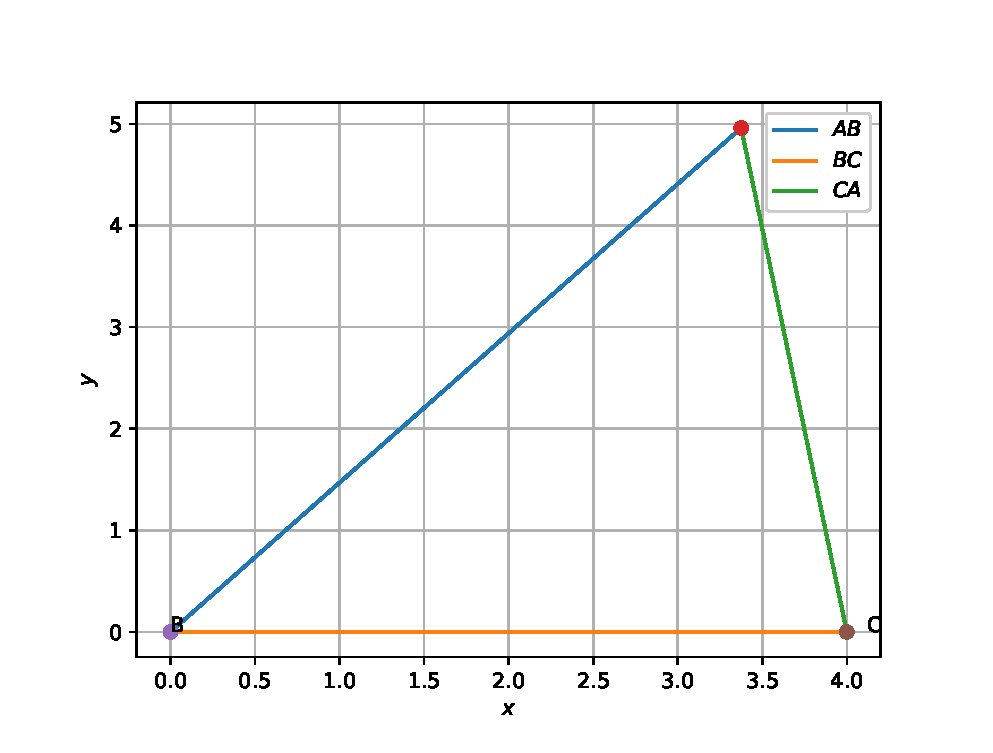
\includegraphics[width=\columnwidth]{./solutions/8/figs/triangle.eps}
\caption{Triangle generated using python}
\label{fig:tri_geo_8_tri_sss_py}
\end{figure}

%
%and the equivalent latex-tikz code generating Fig. \ref{fig:tri_geo_8_tri_right_angle} is 
%\begin{lstlisting}
%figs/triangle.tex
%\end{lstlisting}
%
%The above latex code can be compiled as a standalone document as
%\begin{lstlisting}
%figs/triangle_fig.tex
%\end{lstlisting}

%

%

%
%

%\end{enumerate}



%Let the balanced version of (\ref{eq:solutions/chem/6ato balance}) be
\begin{align}
    \label{eq:solutions/chem/6abalanced}x_{1}HNO_{3}+ x_{2}Ca(OH)_{2}\to x_{3}Ca(NO_{3})_{2}+ x_{4}H_{2}O
\end{align}

which results in the following equations:
\begin{align}
    (x_{1}+ 2x_{2}-2x_{4}) H= 0\\
    (x_{1}-2x_{3}) N= 0\\
    (3x_{1}+ 2x_{2}-6x_{3}- x_{4}) O=0\\
    (x_{2}-x_{3}) Ca= 0
\end{align}

which can be expressed as
\begin{align}
    x_{1}+ 2x_{2}+ 0.x_{3} -2x_{4} = 0\\
    x_{1}+ 0.x_{2} -2x_{3} +0.x_{4}= 0\\
    3x_{1}+ 2x_{2}-6x_{3}- x_{4} =0\\
    0.x_{1} +x_{2}-x_{3} +0.x_{4}= 0
\end{align}

resulting in the matrix equation
\begin{align}
    \label{eq:solutions/chem/6a matrix}
    \myvec{1 & 2 & 0 & -2\\
           1 & 0 & -2 & 0\\
           3 & 2 & -6 & -1\\
           0 & 1 & -1 & 0}\vec{x}
           =\vec{0}
\end{align}

where,
\begin{align}
   \vec{x}= \myvec{x_{1}\\x_{2}\\x_{3}\\x_{4}}
\end{align}

(\ref{eq:solutions/chem/6a matrix}) can be reduced as follows:
\begin{align}
    \myvec{1 & 2 & 0 & -2\\
           1 & 0 & -2 & 0\\
           3 & 2 & -6 & -1\\
           0 & 1 & -1 & 0}
    \xleftrightarrow[R_{3}\leftarrow \frac{R_3}{3}-R_{1}]{R_{2}\leftarrow R_2- R_1}
    \myvec{1 & 2 & 0 & -2\\
           0 & -2 & -2 & 2\\
           0 & -\frac{4}{3} & -2 & \frac{5}{3}\\
           0 & 1 & -1 & 0}\\
    \xleftrightarrow{R_2 \leftarrow -\frac{R_2}{2}}
    \myvec{1 & 2 & 0 & -2\\
          0 & 1 & 1 & -1\\
          0 & -\frac{4}{3} & -2 & \frac{5}{3}\\
          0 & 1 & -1 & 0}\\
    \xleftrightarrow[R_4 \leftarrow R_4- R_2]{R_3 \leftarrow R_3 + \frac{4}{3}R_2}
    \myvec{1 & 2 & 0 & -2\\
           0 & 1 & 1 & -1\\
           0 & 0 & -\frac{2}{3} & \frac{1}{3}\\
           0 & 0 & -2 & 1}\\
    \xleftrightarrow[R_3 \leftarrow -\frac{3}{2}R_3]{R_1 \leftarrow R_1- 2R_2}
    \myvec{1 & 0 & -2 & 0\\
           0 & 1 & 1 & -1\\
           0 & 0 & 1 & -\frac{1}{2}\\
           0 & 0 & -2 & 1}\\
    \xleftrightarrow{R_4\leftarrow R_4 + 2R_3}
    \myvec{1 & 0 & -2 & 0\\
           0 & 1 & 1 & -1\\
           0 & 0 & 1 & -\frac{1}{2}\\
           0 & 0 & 0 & 0}\\
    \xleftrightarrow[R_2\leftarrow R_2-R_3]{R_1\leftarrow R_1 + 2R_3}
    \myvec{1 & 0 & 0 & -1\\
           0 & 1 & 0 & -\frac{1}{2}\\
           0 & 0 & 1 & -\frac{1}{2}\\
           0 & 0 & 0 & 0}
\end{align}

Thus,
\begin{align}
    x_1=x_4, x_2= \frac{1}{2}x_4, x_3=\frac{1}{2}x_4\\
    \implies \quad\vec{x}= x_4\myvec{1\\ \frac{1}{2}\\ \frac{1}{2}\\1} =\myvec{2\\1\\1\\2}
\end{align} 
by substituting $x_4= 2$.

\hfill\break
%\vspace{5mm} 
Hence, (\ref{eq:solutions/chem/6abalanced}) finally becomes
\begin{align}
    2HNO_{3}+ Ca(OH)_{2}\to Ca(NO_{3})_{2}+ 2H_{2}O
\end{align}

%\end{enumerate}

\item  Equal chords of a circle (or of congruent circles) subtend equal angles at the centre. 
\item  If the angles subtended by two chords of a circle (or of congruent circles) at the centre (corresponding centres) are equal, the chords are equal.
\item  The perpendicular from the centre of a circle to a chord bisects the chord. 
\item  The line drawn through the centre of a circle to bisect a chord is perpendicular to the chord.
\item  There is one and only one circle passing through three non-collinear points. 
\item  Equal chords of a circle (or of congruent circles) are equidistant from the centre (or corresponding centres).
\item Chords equidistant from the centre (or corresponding centres) of a circle (or of congruent circles) are equal.
\item  If two arcs of a circle are congruent, then their corresponding chords are equal and conversely if two chords of a circle are equal, then their corresponding arcs (minor, major) are congruent.
\item Congruent arcs of a circle subtend equal angles at the centre. 
\item  The angle subtended by an arc at the centre is double the angle subtended by it at any point on the remaining part of the circle.
\item Angles in the same segment of a circle are equal. \item  Angle in a semicircle is a right angle. 
\item  If a line segment joining two points subtends equal angles at two other points lying on the same side of the line containing the line segment, the four points lie on a circle. 
\item  The sum of either pair of opposite angles of a cyclic quadrilateral is 180$\degree$.
\item  If sum of a pair of opposite angles of a quadrilateral is 180$\degree$, the quadrilateral is cyclic.
%
\item AB is a diameter of the circle, $CD$ is a chord equal to the radius of the circle. $AC$ and $BD$ when extended intersect at a point $E$. Prove that $\angle AEB = 60\degree$.
\item Two circles intersect at two points $A$ and $B$. $AD$ and $AC$ are diameters to the two circles. Prove that $B$ lies on the line segment $DC$.
\item Prove that the quadrilateral formed (if possible) by the internal angle bisectors of any quadrilateral is cyclic.
\item  If two equal chords of a circle intersect within the circle, prove that the segments of one chord are equal to corresponding segments of the other chord.
\item If two equal chords of a circle intersect within the circle, prove that the line joining the point of intersection to the centre makes equal angles with the chords.
%\begin{enumerate}
%The  following Python code generates Fig. \ref{fig:tri_geo_8_tri_sss_py}
%
\begin{lstlisting}
codes/triangle.py
\end{lstlisting}
%\renewcommand{\theequation}{\theenumi}
%\begin{enumerate}[label=\thesection.\arabic*.,ref=\thesection.\theenumi]
%\numberwithin{equation}{enumi}
%\item The figure for the triangle obtained in the question looks like Fig. \ref{fig:tri_geo_8_tri_right_angle}.
%%with angles $\phase{ A},\phase{ C}$ and $\phase{ B}$ and sides $a, b$ and $c$.  The unique feature of this triangle is $\phase{ C}$ which is defined to be $90\degree$.
%with vertices A,B and C
%
%
%%\renewcommand{\thefigure}{\theenumi.\arabic{figure}}
%\begin{figure}[!ht]
%\centering
%\resizebox{\columnwidth}{!}{%\documentclass{standalone}
%
%\usepackage{tikz,pgf} %and any other packages or tikzlibraries your picture needs
%
%\begin{document}
%\resizebox{\columnwidth}{!}{
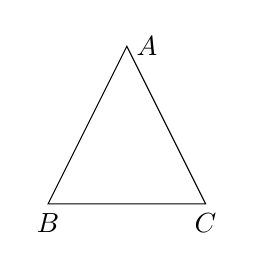
\begin{tikzpicture}
\draw (0,0) node[anchor=north]{$B$}
  -- (1,2) node[anchor=west]{$A$}
  -- (2,0) node[anchor=north]{$C$}
  -- cycle;
\end{tikzpicture}
%}
%\end{document}}
%\caption{Scalene Triangle by Latex-Tikz}
%\label{fig:tri_geo_8_tri_right_angle}	
%\end{figure}
%%
%%
%%\renewcommand{\thefigure}{\theenumi}
%%
%\item List the design parameters for construction
%\label{const:table1}
%\\
%\solution See Table. \ref{table:table1}. 
%%
%\begin{table}[ht!]
%\centering
%%\begin{tabular}{ |p{3cm}|p{3cm}|  }
%%\hline
%% \multicolumn{2}{|c|}{Initial Input Values.} \\
%%\hline
%%a & 4\\
%%\hline
%%b & 3\\
%%\hline
%%$\phase{(ACB)$ & $90^{\circ}$ \\
%%\hline
%%\end{tabular}
%%%%%%%%%%%%%%%%%%%%%%%%%%%%%%%%%%%%%%%%%%%%%%%%%%%%%%%%%%%%%%%%%%%%%%%
%%                                                                  %%
%%  This is the header of a LaTeX2e file exported from Gnumeric.    %%
%%                                                                  %%
%%  This file can be compiled as it stands or included in another   %%
%%  LaTeX document. The table is based on the longtable package so  %%
%%  the longtable options (headers, footers...) can be set in the   %%
%%  preamble section below (see PRAMBLE).                           %%
%%                                                                  %%
%%  To include the file in another, the following two lines must be %%
%%  in the including file:                                          %%
%%        \def\inputGnumericTable{}                                 %%
%%  at the beginning of the file and:                               %%
%%        \input{name-of-this-file.tex}                             %%
%%  where the table is to be placed. Note also that the including   %%
%%  file must use the following packages for the table to be        %%
%%  rendered correctly:                                             %%
%%    \usepackage[latin1]{inputenc}                                 %%
%%    \usepackage{color}                                            %%
%%    \usepackage{array}                                            %%
%%    \usepackage{longtable}                                        %%
%%    \usepackage{calc}                                             %%
%%    \usepackage{multirow}                                         %%
%%    \usepackage{hhline}                                           %%
%%    \usepackage{ifthen}                                           %%
%%  optionally (for landscape tables embedded in another document): %%
%%    \usepackage{lscape}                                           %%
%%                                                                  %%
%%%%%%%%%%%%%%%%%%%%%%%%%%%%%%%%%%%%%%%%%%%%%%%%%%%%%%%%%%%%%%%%%%%%%%



%%  This section checks if we are begin input into another file or  %%
%%  the file will be compiled alone. First use a macro taken from   %%
%%  the TeXbook ex 7.7 (suggestion of Han-Wen Nienhuys).            %%
\def\ifundefined#1{\expandafter\ifx\csname#1\endcsname\relax}


%%  Check for the \def token for inputed files. If it is not        %%
%%  defined, the file will be processed as a standalone and the     %%
%%  preamble will be used.                                          %%
\ifundefined{inputGnumericTable}

%%  We must be able to close or not the document at the end.        %%
	\def\gnumericTableEnd{\end{document}}


%%%%%%%%%%%%%%%%%%%%%%%%%%%%%%%%%%%%%%%%%%%%%%%%%%%%%%%%%%%%%%%%%%%%%%
%%                                                                  %%
%%  This is the PREAMBLE. Change these values to get the right      %%
%%  paper size and other niceties.                                  %%
%%                                                                  %%
%%%%%%%%%%%%%%%%%%%%%%%%%%%%%%%%%%%%%%%%%%%%%%%%%%%%%%%%%%%%%%%%%%%%%%

	\documentclass[12pt%
			  %,landscape%
                    ]{report}
       \usepackage[latin1]{inputenc}
       \usepackage{fullpage}
       \usepackage{color}
       \usepackage{array}
       \usepackage{longtable}
       \usepackage{calc}
       \usepackage{multirow}
       \usepackage{hhline}
       \usepackage{ifthen}
        \usepackage[cmex10]{amsmath}
       \newcommand{\myvec}[1]{\ensuremath{\begin{pmatrix}#1\end{pmatrix}}}

	\begin{document}


%%  End of the preamble for the standalone. The next section is for %%
%%  documents which are included into other LaTeX2e files.          %%
\else

%%  We are not a stand alone document. For a regular table, we will %%
%%  have no preamble and only define the closing to mean nothing.   %%
    \def\gnumericTableEnd{}

%%  If we want landscape mode in an embedded document, comment out  %%
%%  the line above and uncomment the two below. The table will      %%
%%  begin on a new page and run in landscape mode.                  %%
%       \def\gnumericTableEnd{\end{landscape}}
%       \begin{landscape}


%%  End of the else clause for this file being \input.              %%
\fi

%%%%%%%%%%%%%%%%%%%%%%%%%%%%%%%%%%%%%%%%%%%%%%%%%%%%%%%%%%%%%%%%%%%%%%
%%                                                                  %%
%%  The rest is the gnumeric table, except for the closing          %%
%%  statement. Changes below will alter the table's appearance.     %%
%%                                                                  %%
%%%%%%%%%%%%%%%%%%%%%%%%%%%%%%%%%%%%%%%%%%%%%%%%%%%%%%%%%%%%%%%%%%%%%%

\providecommand{\gnumericmathit}[1]{#1} 
%%  Uncomment the next line if you would like your numbers to be in %%
%%  italics if they are italizised in the gnumeric table.           %%
%\renewcommand{\gnumericmathit}[1]{\mathit{#1}}
\providecommand{\gnumericPB}[1]%
{\let\gnumericTemp=\\#1\let\\=\gnumericTemp\hspace{0pt}}
 \ifundefined{gnumericTableWidthDefined}
        \newlength{\gnumericTableWidth}
        \newlength{\gnumericTableWidthComplete}
        \newlength{\gnumericMultiRowLength}
        \global\def\gnumericTableWidthDefined{}
 \fi
%% The following setting protects this code from babel shorthands.  %%
 \ifthenelse{\isundefined{\languageshorthands}}{}{\languageshorthands{english}}
%%  The default table format retains the relative column widths of  %%
%%  gnumeric. They can easily be changed to c, r or l. In that case %%
%%  you may want to comment out the next line and uncomment the one %%
%%  thereafter                                                      %%
\providecommand\gnumbox{\makebox[0pt]}
%%\providecommand\gnumbox[1][]{\makebox}

%% to adjust positions in multirow situations                       %%
\setlength{\bigstrutjot}{\jot}
\setlength{\extrarowheight}{\doublerulesep}

%%  The \setlongtables command keeps column widths the same across  %%
%%  pages. Simply comment out next line for varying column widths.  %%
\setlongtables

\setlength\gnumericTableWidth{%
	71pt+%
	95pt+%
0pt}
\def\gumericNumCols{2}
\setlength\gnumericTableWidthComplete{\gnumericTableWidth+%
         \tabcolsep*\gumericNumCols*2+\arrayrulewidth*\gumericNumCols}
\ifthenelse{\lengthtest{\gnumericTableWidthComplete > \linewidth}}%
         {\def\gnumericScale{\ratio{\linewidth-%
                        \tabcolsep*\gumericNumCols*2-%
                        \arrayrulewidth*\gumericNumCols}%
{\gnumericTableWidth}}}%
{\def\gnumericScale{1}}

%%%%%%%%%%%%%%%%%%%%%%%%%%%%%%%%%%%%%%%%%%%%%%%%%%%%%%%%%%%%%%%%%%%%%%
%%                                                                  %%
%% The following are the widths of the various columns. We are      %%
%% defining them here because then they are easier to change.       %%
%% Depending on the cell formats we may use them more than once.    %%
%%                                                                  %%
%%%%%%%%%%%%%%%%%%%%%%%%%%%%%%%%%%%%%%%%%%%%%%%%%%%%%%%%%%%%%%%%%%%%%%

\ifthenelse{\isundefined{\gnumericColA}}{\newlength{\gnumericColA}}{}\settowidth{\gnumericColA}{\begin{tabular}{@{}p{71pt*\gnumericScale}@{}}x\end{tabular}}
\ifthenelse{\isundefined{\gnumericColB}}{\newlength{\gnumericColB}}{}\settowidth{\gnumericColB}{\begin{tabular}{@{}p{95pt*\gnumericScale}@{}}x\end{tabular}}

\begin{tabular}[c]{%
	b{\gnumericColA}%
	b{\gnumericColB}%
	}

%%%%%%%%%%%%%%%%%%%%%%%%%%%%%%%%%%%%%%%%%%%%%%%%%%%%%%%%%%%%%%%%%%%%%%
%%  The longtable options. (Caption, headers... see Goosens, p.124) %%
%	\caption{The Table Caption.}             \\	%
% \hline	% Across the top of the table.
%%  The rest of these options are table rows which are placed on    %%
%%  the first, last or every page. Use \multicolumn if you want.    %%

%%  Header for the first page.                                      %%
%	\multicolumn{2}{c}{The First Header} \\ \hline 
%	\multicolumn{1}{c}{colTag}	%Column 1
%	&\multicolumn{1}{c}{colTag}	\\ \hline %Last column
%	\endfirsthead

%%  The running header definition.                                  %%
%	\hline
%	\multicolumn{2}{l}{\ldots\small\slshape continued} \\ \hline
%	\multicolumn{1}{c}{colTag}	%Column 1
%	&\multicolumn{1}{c}{colTag}	\\ \hline %Last column
%	\endhead

%%  The running footer definition.                                  %%
%	\hline
%	\multicolumn{2}{r}{\small\slshape continued\ldots} \\
%	\endfoot

%%  The ending footer definition.                                   %%
%	\multicolumn{2}{c}{That's all folks} \\ \hline 
%	\endlastfoot
%%%%%%%%%%%%%%%%%%%%%%%%%%%%%%%%%%%%%%%%%%%%%%%%%%%%%%%%%%%%%%%%%%%%%%

\hhline{|--}
	 \multicolumn{2}{|p{	\gnumericColA+%
	\gnumericColB+%
	\tabcolsep*2*1}|}%
	{\gnumericPB{\centering}\gnumbox{Input values}}
\\
\hhline{|-|-|}
	 \multicolumn{1}{|p{\gnumericColA}|}%
	{\gnumericPB{\centering}\gnumbox{Parameters}}
	&\multicolumn{1}{p{\gnumericColB}|}%
	{\gnumericPB{\centering}\gnumbox{Values}}
\\
\hhline{|--|}
	 \multicolumn{1}{|p{\gnumericColA}|}%
	{\gnumericPB{\centering}\gnumbox{\textbf{O}}}
	&\multicolumn{1}{p{\gnumericColB}|}%
	{$\myvec{2\\-3}$}
\\
\hhline{|--|}
	 \multicolumn{1}{|p{\gnumericColA}|}%
	{\gnumericPB{\centering}\gnumbox{\textbf{A}}}
	&\multicolumn{1}{p{\gnumericColB}|}%
	{$\myvec{1\\4}$}
\\
\hhline{|-|-|}
\end{tabular}

\ifthenelse{\isundefined{\languageshorthands}}{}{\languageshorthands{\languagename}}
\gnumericTableEnd

%\caption{To construct $\triangle ABC$}
%\label{table:table1}	
%\end{table}
%
%%\item
%%	For simplicity, let the greek letter $\alpha = \phase{ B$.  We have the following definitions.
%%\begin{equation}
%%\label{eq:tri_trig_defs}
%%\begin{matrix}
%	%\sin \theta = \frac{b}{c} & 	\cos \theta = \frac{a}{c} \\
%	%\tan \theta = \frac{c}{a} & \cot \theta = \frac{1}{\tan \theta} \\
%	%\csc \theta = \frac{1}{\sin \theta} & \sec \theta = \frac{1}{\cos \theta}
%	%\end{equation}
%%
%\item Find the coordinates of the various points in Fig. \ref{fig:tri_geo_8_tri_right_angle}
%\label{const:tri_right_angle}
%\\
%
%\solution 
From the given information, 
%$\triangle ABC$ are 
\begin{align}
\label{eq:constr_a}
\vec{A} &= \myvec{4\\-6} 
\\
\vec{B} &= \myvec{3\\-2}, 
\label{eq:constr_b}
\\
\vec{C} &= \myvec{5\\2}
\label{eq:constr_c}
\end{align}
$\because \vec{M}$ is the midpoint of $AB$,
\begin{align}
\vec{M}= \frac{\vec{A}+\vec{B}}{2} = \frac{1}{2}\myvec{7\\-8}
\label{eq:constr_m}
\end{align}

$\because \vec{N}$ is the midpoint of $BC$,
\begin{align}
\vec{N}= \frac{\vec{B}+\vec{C}}{2} = \frac{1}{2}\myvec{8\\0}
\label{eq:constr_n}
\end{align}

$\because \vec{P}$ is the midpoint of $CA$,
\begin{align}
\vec{P}= \frac{\vec{C}+\vec{A}}{2} = \frac{1}{2}\myvec{9\\-4}
\label{eq:constr_p}
\end{align}
%
%Also, $\vec{M}$ is given to be the midpoint of $C$.  Hence, 
%\begin{align}
%\vec{M}&= \frac{\vec{C}+\vec{D}}{2}
%\\
%\implies \vec{D} &= 2 \vec{M} - \vec{C} = \myvec{a\\b}
%\label{eq:constr_d}
%\end{align}
%
%The values are listed in 
%%\item List the  derived values.
%%\label{const:table2}
%%\\
%%\solution See  
%Table. \ref{table:table2} 
%\begin{table}[ht!]
%\centering
%\begin{tabular}{ |p{3cm}|p{3cm}|  }
%\hline
% \multicolumn{2}{|c|}{Derived Values.} \\
%\hline
%$\vec{M}$ & $$\begin{pmatrix}3.5\\-4\end{pmatrix}$$\\						
%\hline
%$\vec{N}$ & $$\begin{pmatrix}4\\0\end{pmatrix} $$\\
%\hline
%$\vec{P}$ & $$\begin{pmatrix}4.5\\-2\end{pmatrix} $$\\
%\hline
%\end{tabular}
%\caption{To get Mid-points of $\triangle ABC$}
%\label{table:table2}
%\end{table}
%
%\item Draw Fig. \ref{fig:tri_geo_8_tri_right_angle}.	
%\\
%\solution 

The  following Python code verifies the determinant values.

\begin{lstlisting}
codes/determinant_check.py
\end{lstlisting}

\begin{figure}[!ht]
\centering
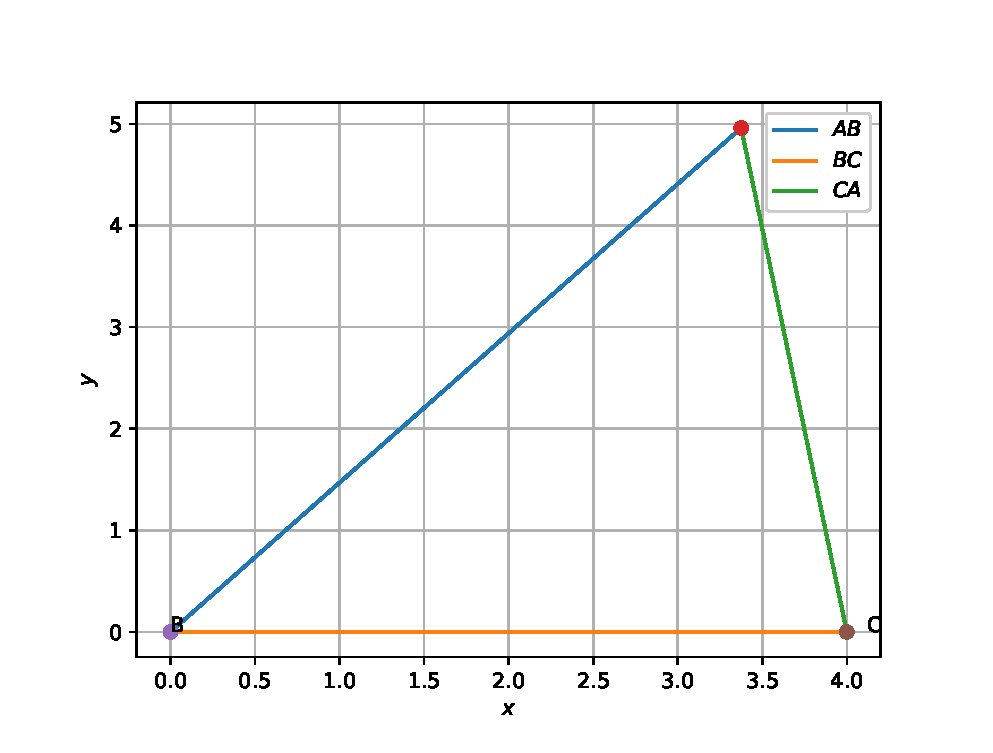
\includegraphics[width=\columnwidth]{./solutions/8/figs/triangle.eps}
\caption{Triangle generated using python}
\label{fig:tri_geo_8_tri_sss_py}
\end{figure}

%
%and the equivalent latex-tikz code generating Fig. \ref{fig:tri_geo_8_tri_right_angle} is 
%\begin{lstlisting}
%figs/triangle.tex
%\end{lstlisting}
%
%The above latex code can be compiled as a standalone document as
%\begin{lstlisting}
%figs/triangle_fig.tex
%\end{lstlisting}

%

%

%
%

%\end{enumerate}



%Let the balanced version of (\ref{eq:solutions/chem/6ato balance}) be
\begin{align}
    \label{eq:solutions/chem/6abalanced}x_{1}HNO_{3}+ x_{2}Ca(OH)_{2}\to x_{3}Ca(NO_{3})_{2}+ x_{4}H_{2}O
\end{align}

which results in the following equations:
\begin{align}
    (x_{1}+ 2x_{2}-2x_{4}) H= 0\\
    (x_{1}-2x_{3}) N= 0\\
    (3x_{1}+ 2x_{2}-6x_{3}- x_{4}) O=0\\
    (x_{2}-x_{3}) Ca= 0
\end{align}

which can be expressed as
\begin{align}
    x_{1}+ 2x_{2}+ 0.x_{3} -2x_{4} = 0\\
    x_{1}+ 0.x_{2} -2x_{3} +0.x_{4}= 0\\
    3x_{1}+ 2x_{2}-6x_{3}- x_{4} =0\\
    0.x_{1} +x_{2}-x_{3} +0.x_{4}= 0
\end{align}

resulting in the matrix equation
\begin{align}
    \label{eq:solutions/chem/6a matrix}
    \myvec{1 & 2 & 0 & -2\\
           1 & 0 & -2 & 0\\
           3 & 2 & -6 & -1\\
           0 & 1 & -1 & 0}\vec{x}
           =\vec{0}
\end{align}

where,
\begin{align}
   \vec{x}= \myvec{x_{1}\\x_{2}\\x_{3}\\x_{4}}
\end{align}

(\ref{eq:solutions/chem/6a matrix}) can be reduced as follows:
\begin{align}
    \myvec{1 & 2 & 0 & -2\\
           1 & 0 & -2 & 0\\
           3 & 2 & -6 & -1\\
           0 & 1 & -1 & 0}
    \xleftrightarrow[R_{3}\leftarrow \frac{R_3}{3}-R_{1}]{R_{2}\leftarrow R_2- R_1}
    \myvec{1 & 2 & 0 & -2\\
           0 & -2 & -2 & 2\\
           0 & -\frac{4}{3} & -2 & \frac{5}{3}\\
           0 & 1 & -1 & 0}\\
    \xleftrightarrow{R_2 \leftarrow -\frac{R_2}{2}}
    \myvec{1 & 2 & 0 & -2\\
          0 & 1 & 1 & -1\\
          0 & -\frac{4}{3} & -2 & \frac{5}{3}\\
          0 & 1 & -1 & 0}\\
    \xleftrightarrow[R_4 \leftarrow R_4- R_2]{R_3 \leftarrow R_3 + \frac{4}{3}R_2}
    \myvec{1 & 2 & 0 & -2\\
           0 & 1 & 1 & -1\\
           0 & 0 & -\frac{2}{3} & \frac{1}{3}\\
           0 & 0 & -2 & 1}\\
    \xleftrightarrow[R_3 \leftarrow -\frac{3}{2}R_3]{R_1 \leftarrow R_1- 2R_2}
    \myvec{1 & 0 & -2 & 0\\
           0 & 1 & 1 & -1\\
           0 & 0 & 1 & -\frac{1}{2}\\
           0 & 0 & -2 & 1}\\
    \xleftrightarrow{R_4\leftarrow R_4 + 2R_3}
    \myvec{1 & 0 & -2 & 0\\
           0 & 1 & 1 & -1\\
           0 & 0 & 1 & -\frac{1}{2}\\
           0 & 0 & 0 & 0}\\
    \xleftrightarrow[R_2\leftarrow R_2-R_3]{R_1\leftarrow R_1 + 2R_3}
    \myvec{1 & 0 & 0 & -1\\
           0 & 1 & 0 & -\frac{1}{2}\\
           0 & 0 & 1 & -\frac{1}{2}\\
           0 & 0 & 0 & 0}
\end{align}

Thus,
\begin{align}
    x_1=x_4, x_2= \frac{1}{2}x_4, x_3=\frac{1}{2}x_4\\
    \implies \quad\vec{x}= x_4\myvec{1\\ \frac{1}{2}\\ \frac{1}{2}\\1} =\myvec{2\\1\\1\\2}
\end{align} 
by substituting $x_4= 2$.

\hfill\break
%\vspace{5mm} 
Hence, (\ref{eq:solutions/chem/6abalanced}) finally becomes
\begin{align}
    2HNO_{3}+ Ca(OH)_{2}\to Ca(NO_{3})_{2}+ 2H_{2}O
\end{align}

%\end{enumerate}

\item If a line intersects two concentric circles (circles with the same centre) with centre O at A, B, C and D, prove that AB = CD.
%\begin{enumerate}
%The  following Python code generates Fig. \ref{fig:tri_geo_8_tri_sss_py}
%
\begin{lstlisting}
codes/triangle.py
\end{lstlisting}
%\renewcommand{\theequation}{\theenumi}
%\begin{enumerate}[label=\thesection.\arabic*.,ref=\thesection.\theenumi]
%\numberwithin{equation}{enumi}
%\item The figure for the triangle obtained in the question looks like Fig. \ref{fig:tri_geo_8_tri_right_angle}.
%%with angles $\phase{ A},\phase{ C}$ and $\phase{ B}$ and sides $a, b$ and $c$.  The unique feature of this triangle is $\phase{ C}$ which is defined to be $90\degree$.
%with vertices A,B and C
%
%
%%\renewcommand{\thefigure}{\theenumi.\arabic{figure}}
%\begin{figure}[!ht]
%\centering
%\resizebox{\columnwidth}{!}{%\documentclass{standalone}
%
%\usepackage{tikz,pgf} %and any other packages or tikzlibraries your picture needs
%
%\begin{document}
%\resizebox{\columnwidth}{!}{
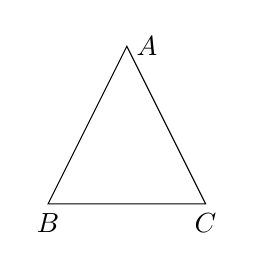
\begin{tikzpicture}
\draw (0,0) node[anchor=north]{$B$}
  -- (1,2) node[anchor=west]{$A$}
  -- (2,0) node[anchor=north]{$C$}
  -- cycle;
\end{tikzpicture}
%}
%\end{document}}
%\caption{Scalene Triangle by Latex-Tikz}
%\label{fig:tri_geo_8_tri_right_angle}	
%\end{figure}
%%
%%
%%\renewcommand{\thefigure}{\theenumi}
%%
%\item List the design parameters for construction
%\label{const:table1}
%\\
%\solution See Table. \ref{table:table1}. 
%%
%\begin{table}[ht!]
%\centering
%%\begin{tabular}{ |p{3cm}|p{3cm}|  }
%%\hline
%% \multicolumn{2}{|c|}{Initial Input Values.} \\
%%\hline
%%a & 4\\
%%\hline
%%b & 3\\
%%\hline
%%$\phase{(ACB)$ & $90^{\circ}$ \\
%%\hline
%%\end{tabular}
%%%%%%%%%%%%%%%%%%%%%%%%%%%%%%%%%%%%%%%%%%%%%%%%%%%%%%%%%%%%%%%%%%%%%%%
%%                                                                  %%
%%  This is the header of a LaTeX2e file exported from Gnumeric.    %%
%%                                                                  %%
%%  This file can be compiled as it stands or included in another   %%
%%  LaTeX document. The table is based on the longtable package so  %%
%%  the longtable options (headers, footers...) can be set in the   %%
%%  preamble section below (see PRAMBLE).                           %%
%%                                                                  %%
%%  To include the file in another, the following two lines must be %%
%%  in the including file:                                          %%
%%        \def\inputGnumericTable{}                                 %%
%%  at the beginning of the file and:                               %%
%%        \input{name-of-this-file.tex}                             %%
%%  where the table is to be placed. Note also that the including   %%
%%  file must use the following packages for the table to be        %%
%%  rendered correctly:                                             %%
%%    \usepackage[latin1]{inputenc}                                 %%
%%    \usepackage{color}                                            %%
%%    \usepackage{array}                                            %%
%%    \usepackage{longtable}                                        %%
%%    \usepackage{calc}                                             %%
%%    \usepackage{multirow}                                         %%
%%    \usepackage{hhline}                                           %%
%%    \usepackage{ifthen}                                           %%
%%  optionally (for landscape tables embedded in another document): %%
%%    \usepackage{lscape}                                           %%
%%                                                                  %%
%%%%%%%%%%%%%%%%%%%%%%%%%%%%%%%%%%%%%%%%%%%%%%%%%%%%%%%%%%%%%%%%%%%%%%



%%  This section checks if we are begin input into another file or  %%
%%  the file will be compiled alone. First use a macro taken from   %%
%%  the TeXbook ex 7.7 (suggestion of Han-Wen Nienhuys).            %%
\def\ifundefined#1{\expandafter\ifx\csname#1\endcsname\relax}


%%  Check for the \def token for inputed files. If it is not        %%
%%  defined, the file will be processed as a standalone and the     %%
%%  preamble will be used.                                          %%
\ifundefined{inputGnumericTable}

%%  We must be able to close or not the document at the end.        %%
	\def\gnumericTableEnd{\end{document}}


%%%%%%%%%%%%%%%%%%%%%%%%%%%%%%%%%%%%%%%%%%%%%%%%%%%%%%%%%%%%%%%%%%%%%%
%%                                                                  %%
%%  This is the PREAMBLE. Change these values to get the right      %%
%%  paper size and other niceties.                                  %%
%%                                                                  %%
%%%%%%%%%%%%%%%%%%%%%%%%%%%%%%%%%%%%%%%%%%%%%%%%%%%%%%%%%%%%%%%%%%%%%%

	\documentclass[12pt%
			  %,landscape%
                    ]{report}
       \usepackage[latin1]{inputenc}
       \usepackage{fullpage}
       \usepackage{color}
       \usepackage{array}
       \usepackage{longtable}
       \usepackage{calc}
       \usepackage{multirow}
       \usepackage{hhline}
       \usepackage{ifthen}
        \usepackage[cmex10]{amsmath}
       \newcommand{\myvec}[1]{\ensuremath{\begin{pmatrix}#1\end{pmatrix}}}

	\begin{document}


%%  End of the preamble for the standalone. The next section is for %%
%%  documents which are included into other LaTeX2e files.          %%
\else

%%  We are not a stand alone document. For a regular table, we will %%
%%  have no preamble and only define the closing to mean nothing.   %%
    \def\gnumericTableEnd{}

%%  If we want landscape mode in an embedded document, comment out  %%
%%  the line above and uncomment the two below. The table will      %%
%%  begin on a new page and run in landscape mode.                  %%
%       \def\gnumericTableEnd{\end{landscape}}
%       \begin{landscape}


%%  End of the else clause for this file being \input.              %%
\fi

%%%%%%%%%%%%%%%%%%%%%%%%%%%%%%%%%%%%%%%%%%%%%%%%%%%%%%%%%%%%%%%%%%%%%%
%%                                                                  %%
%%  The rest is the gnumeric table, except for the closing          %%
%%  statement. Changes below will alter the table's appearance.     %%
%%                                                                  %%
%%%%%%%%%%%%%%%%%%%%%%%%%%%%%%%%%%%%%%%%%%%%%%%%%%%%%%%%%%%%%%%%%%%%%%

\providecommand{\gnumericmathit}[1]{#1} 
%%  Uncomment the next line if you would like your numbers to be in %%
%%  italics if they are italizised in the gnumeric table.           %%
%\renewcommand{\gnumericmathit}[1]{\mathit{#1}}
\providecommand{\gnumericPB}[1]%
{\let\gnumericTemp=\\#1\let\\=\gnumericTemp\hspace{0pt}}
 \ifundefined{gnumericTableWidthDefined}
        \newlength{\gnumericTableWidth}
        \newlength{\gnumericTableWidthComplete}
        \newlength{\gnumericMultiRowLength}
        \global\def\gnumericTableWidthDefined{}
 \fi
%% The following setting protects this code from babel shorthands.  %%
 \ifthenelse{\isundefined{\languageshorthands}}{}{\languageshorthands{english}}
%%  The default table format retains the relative column widths of  %%
%%  gnumeric. They can easily be changed to c, r or l. In that case %%
%%  you may want to comment out the next line and uncomment the one %%
%%  thereafter                                                      %%
\providecommand\gnumbox{\makebox[0pt]}
%%\providecommand\gnumbox[1][]{\makebox}

%% to adjust positions in multirow situations                       %%
\setlength{\bigstrutjot}{\jot}
\setlength{\extrarowheight}{\doublerulesep}

%%  The \setlongtables command keeps column widths the same across  %%
%%  pages. Simply comment out next line for varying column widths.  %%
\setlongtables

\setlength\gnumericTableWidth{%
	71pt+%
	95pt+%
0pt}
\def\gumericNumCols{2}
\setlength\gnumericTableWidthComplete{\gnumericTableWidth+%
         \tabcolsep*\gumericNumCols*2+\arrayrulewidth*\gumericNumCols}
\ifthenelse{\lengthtest{\gnumericTableWidthComplete > \linewidth}}%
         {\def\gnumericScale{\ratio{\linewidth-%
                        \tabcolsep*\gumericNumCols*2-%
                        \arrayrulewidth*\gumericNumCols}%
{\gnumericTableWidth}}}%
{\def\gnumericScale{1}}

%%%%%%%%%%%%%%%%%%%%%%%%%%%%%%%%%%%%%%%%%%%%%%%%%%%%%%%%%%%%%%%%%%%%%%
%%                                                                  %%
%% The following are the widths of the various columns. We are      %%
%% defining them here because then they are easier to change.       %%
%% Depending on the cell formats we may use them more than once.    %%
%%                                                                  %%
%%%%%%%%%%%%%%%%%%%%%%%%%%%%%%%%%%%%%%%%%%%%%%%%%%%%%%%%%%%%%%%%%%%%%%

\ifthenelse{\isundefined{\gnumericColA}}{\newlength{\gnumericColA}}{}\settowidth{\gnumericColA}{\begin{tabular}{@{}p{71pt*\gnumericScale}@{}}x\end{tabular}}
\ifthenelse{\isundefined{\gnumericColB}}{\newlength{\gnumericColB}}{}\settowidth{\gnumericColB}{\begin{tabular}{@{}p{95pt*\gnumericScale}@{}}x\end{tabular}}

\begin{tabular}[c]{%
	b{\gnumericColA}%
	b{\gnumericColB}%
	}

%%%%%%%%%%%%%%%%%%%%%%%%%%%%%%%%%%%%%%%%%%%%%%%%%%%%%%%%%%%%%%%%%%%%%%
%%  The longtable options. (Caption, headers... see Goosens, p.124) %%
%	\caption{The Table Caption.}             \\	%
% \hline	% Across the top of the table.
%%  The rest of these options are table rows which are placed on    %%
%%  the first, last or every page. Use \multicolumn if you want.    %%

%%  Header for the first page.                                      %%
%	\multicolumn{2}{c}{The First Header} \\ \hline 
%	\multicolumn{1}{c}{colTag}	%Column 1
%	&\multicolumn{1}{c}{colTag}	\\ \hline %Last column
%	\endfirsthead

%%  The running header definition.                                  %%
%	\hline
%	\multicolumn{2}{l}{\ldots\small\slshape continued} \\ \hline
%	\multicolumn{1}{c}{colTag}	%Column 1
%	&\multicolumn{1}{c}{colTag}	\\ \hline %Last column
%	\endhead

%%  The running footer definition.                                  %%
%	\hline
%	\multicolumn{2}{r}{\small\slshape continued\ldots} \\
%	\endfoot

%%  The ending footer definition.                                   %%
%	\multicolumn{2}{c}{That's all folks} \\ \hline 
%	\endlastfoot
%%%%%%%%%%%%%%%%%%%%%%%%%%%%%%%%%%%%%%%%%%%%%%%%%%%%%%%%%%%%%%%%%%%%%%

\hhline{|--}
	 \multicolumn{2}{|p{	\gnumericColA+%
	\gnumericColB+%
	\tabcolsep*2*1}|}%
	{\gnumericPB{\centering}\gnumbox{Input values}}
\\
\hhline{|-|-|}
	 \multicolumn{1}{|p{\gnumericColA}|}%
	{\gnumericPB{\centering}\gnumbox{Parameters}}
	&\multicolumn{1}{p{\gnumericColB}|}%
	{\gnumericPB{\centering}\gnumbox{Values}}
\\
\hhline{|--|}
	 \multicolumn{1}{|p{\gnumericColA}|}%
	{\gnumericPB{\centering}\gnumbox{\textbf{O}}}
	&\multicolumn{1}{p{\gnumericColB}|}%
	{$\myvec{2\\-3}$}
\\
\hhline{|--|}
	 \multicolumn{1}{|p{\gnumericColA}|}%
	{\gnumericPB{\centering}\gnumbox{\textbf{A}}}
	&\multicolumn{1}{p{\gnumericColB}|}%
	{$\myvec{1\\4}$}
\\
\hhline{|-|-|}
\end{tabular}

\ifthenelse{\isundefined{\languageshorthands}}{}{\languageshorthands{\languagename}}
\gnumericTableEnd

%\caption{To construct $\triangle ABC$}
%\label{table:table1}	
%\end{table}
%
%%\item
%%	For simplicity, let the greek letter $\alpha = \phase{ B$.  We have the following definitions.
%%\begin{equation}
%%\label{eq:tri_trig_defs}
%%\begin{matrix}
%	%\sin \theta = \frac{b}{c} & 	\cos \theta = \frac{a}{c} \\
%	%\tan \theta = \frac{c}{a} & \cot \theta = \frac{1}{\tan \theta} \\
%	%\csc \theta = \frac{1}{\sin \theta} & \sec \theta = \frac{1}{\cos \theta}
%	%\end{equation}
%%
%\item Find the coordinates of the various points in Fig. \ref{fig:tri_geo_8_tri_right_angle}
%\label{const:tri_right_angle}
%\\
%
%\solution 
From the given information, 
%$\triangle ABC$ are 
\begin{align}
\label{eq:constr_a}
\vec{A} &= \myvec{4\\-6} 
\\
\vec{B} &= \myvec{3\\-2}, 
\label{eq:constr_b}
\\
\vec{C} &= \myvec{5\\2}
\label{eq:constr_c}
\end{align}
$\because \vec{M}$ is the midpoint of $AB$,
\begin{align}
\vec{M}= \frac{\vec{A}+\vec{B}}{2} = \frac{1}{2}\myvec{7\\-8}
\label{eq:constr_m}
\end{align}

$\because \vec{N}$ is the midpoint of $BC$,
\begin{align}
\vec{N}= \frac{\vec{B}+\vec{C}}{2} = \frac{1}{2}\myvec{8\\0}
\label{eq:constr_n}
\end{align}

$\because \vec{P}$ is the midpoint of $CA$,
\begin{align}
\vec{P}= \frac{\vec{C}+\vec{A}}{2} = \frac{1}{2}\myvec{9\\-4}
\label{eq:constr_p}
\end{align}
%
%Also, $\vec{M}$ is given to be the midpoint of $C$.  Hence, 
%\begin{align}
%\vec{M}&= \frac{\vec{C}+\vec{D}}{2}
%\\
%\implies \vec{D} &= 2 \vec{M} - \vec{C} = \myvec{a\\b}
%\label{eq:constr_d}
%\end{align}
%
%The values are listed in 
%%\item List the  derived values.
%%\label{const:table2}
%%\\
%%\solution See  
%Table. \ref{table:table2} 
%\begin{table}[ht!]
%\centering
%\begin{tabular}{ |p{3cm}|p{3cm}|  }
%\hline
% \multicolumn{2}{|c|}{Derived Values.} \\
%\hline
%$\vec{M}$ & $$\begin{pmatrix}3.5\\-4\end{pmatrix}$$\\						
%\hline
%$\vec{N}$ & $$\begin{pmatrix}4\\0\end{pmatrix} $$\\
%\hline
%$\vec{P}$ & $$\begin{pmatrix}4.5\\-2\end{pmatrix} $$\\
%\hline
%\end{tabular}
%\caption{To get Mid-points of $\triangle ABC$}
%\label{table:table2}
%\end{table}
%
%\item Draw Fig. \ref{fig:tri_geo_8_tri_right_angle}.	
%\\
%\solution 

The  following Python code verifies the determinant values.

\begin{lstlisting}
codes/determinant_check.py
\end{lstlisting}

\begin{figure}[!ht]
\centering
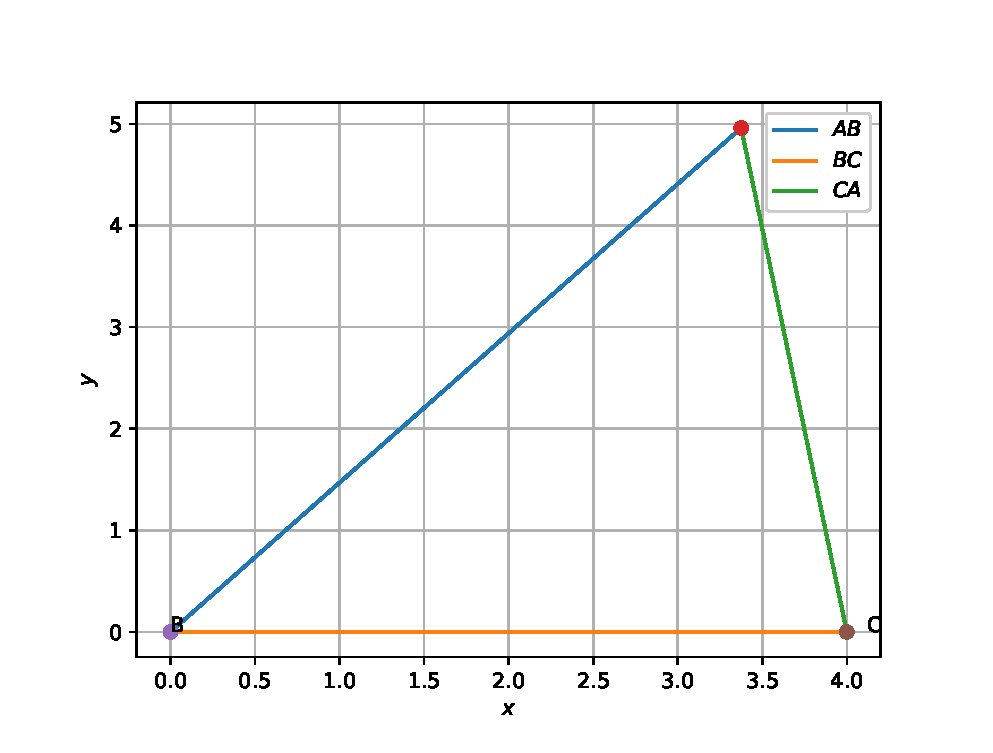
\includegraphics[width=\columnwidth]{./solutions/8/figs/triangle.eps}
\caption{Triangle generated using python}
\label{fig:tri_geo_8_tri_sss_py}
\end{figure}

%
%and the equivalent latex-tikz code generating Fig. \ref{fig:tri_geo_8_tri_right_angle} is 
%\begin{lstlisting}
%figs/triangle.tex
%\end{lstlisting}
%
%The above latex code can be compiled as a standalone document as
%\begin{lstlisting}
%figs/triangle_fig.tex
%\end{lstlisting}

%

%

%
%

%\end{enumerate}



%Let the balanced version of (\ref{eq:solutions/chem/6ato balance}) be
\begin{align}
    \label{eq:solutions/chem/6abalanced}x_{1}HNO_{3}+ x_{2}Ca(OH)_{2}\to x_{3}Ca(NO_{3})_{2}+ x_{4}H_{2}O
\end{align}

which results in the following equations:
\begin{align}
    (x_{1}+ 2x_{2}-2x_{4}) H= 0\\
    (x_{1}-2x_{3}) N= 0\\
    (3x_{1}+ 2x_{2}-6x_{3}- x_{4}) O=0\\
    (x_{2}-x_{3}) Ca= 0
\end{align}

which can be expressed as
\begin{align}
    x_{1}+ 2x_{2}+ 0.x_{3} -2x_{4} = 0\\
    x_{1}+ 0.x_{2} -2x_{3} +0.x_{4}= 0\\
    3x_{1}+ 2x_{2}-6x_{3}- x_{4} =0\\
    0.x_{1} +x_{2}-x_{3} +0.x_{4}= 0
\end{align}

resulting in the matrix equation
\begin{align}
    \label{eq:solutions/chem/6a matrix}
    \myvec{1 & 2 & 0 & -2\\
           1 & 0 & -2 & 0\\
           3 & 2 & -6 & -1\\
           0 & 1 & -1 & 0}\vec{x}
           =\vec{0}
\end{align}

where,
\begin{align}
   \vec{x}= \myvec{x_{1}\\x_{2}\\x_{3}\\x_{4}}
\end{align}

(\ref{eq:solutions/chem/6a matrix}) can be reduced as follows:
\begin{align}
    \myvec{1 & 2 & 0 & -2\\
           1 & 0 & -2 & 0\\
           3 & 2 & -6 & -1\\
           0 & 1 & -1 & 0}
    \xleftrightarrow[R_{3}\leftarrow \frac{R_3}{3}-R_{1}]{R_{2}\leftarrow R_2- R_1}
    \myvec{1 & 2 & 0 & -2\\
           0 & -2 & -2 & 2\\
           0 & -\frac{4}{3} & -2 & \frac{5}{3}\\
           0 & 1 & -1 & 0}\\
    \xleftrightarrow{R_2 \leftarrow -\frac{R_2}{2}}
    \myvec{1 & 2 & 0 & -2\\
          0 & 1 & 1 & -1\\
          0 & -\frac{4}{3} & -2 & \frac{5}{3}\\
          0 & 1 & -1 & 0}\\
    \xleftrightarrow[R_4 \leftarrow R_4- R_2]{R_3 \leftarrow R_3 + \frac{4}{3}R_2}
    \myvec{1 & 2 & 0 & -2\\
           0 & 1 & 1 & -1\\
           0 & 0 & -\frac{2}{3} & \frac{1}{3}\\
           0 & 0 & -2 & 1}\\
    \xleftrightarrow[R_3 \leftarrow -\frac{3}{2}R_3]{R_1 \leftarrow R_1- 2R_2}
    \myvec{1 & 0 & -2 & 0\\
           0 & 1 & 1 & -1\\
           0 & 0 & 1 & -\frac{1}{2}\\
           0 & 0 & -2 & 1}\\
    \xleftrightarrow{R_4\leftarrow R_4 + 2R_3}
    \myvec{1 & 0 & -2 & 0\\
           0 & 1 & 1 & -1\\
           0 & 0 & 1 & -\frac{1}{2}\\
           0 & 0 & 0 & 0}\\
    \xleftrightarrow[R_2\leftarrow R_2-R_3]{R_1\leftarrow R_1 + 2R_3}
    \myvec{1 & 0 & 0 & -1\\
           0 & 1 & 0 & -\frac{1}{2}\\
           0 & 0 & 1 & -\frac{1}{2}\\
           0 & 0 & 0 & 0}
\end{align}

Thus,
\begin{align}
    x_1=x_4, x_2= \frac{1}{2}x_4, x_3=\frac{1}{2}x_4\\
    \implies \quad\vec{x}= x_4\myvec{1\\ \frac{1}{2}\\ \frac{1}{2}\\1} =\myvec{2\\1\\1\\2}
\end{align} 
by substituting $x_4= 2$.

\hfill\break
%\vspace{5mm} 
Hence, (\ref{eq:solutions/chem/6abalanced}) finally becomes
\begin{align}
    2HNO_{3}+ Ca(OH)_{2}\to Ca(NO_{3})_{2}+ 2H_{2}O
\end{align}

%\end{enumerate}
\item A chord of a circle is equal to the radius of the
circle. Find the angle subtended by the chord at
a point on the minor arc and also at a point on the
major arc.
\item If diagonals of a cyclic quadrilateral are diameters of the circle through the vertices of
the quadrilateral, prove that it is a rectangle.
\item If the non-parallel sides of a trapezium are equal, prove that it is cyclic.
%\begin{enumerate}
%\renewcommand{\theequation}{\theenumi}
\begin{enumerate}[label=\thesection.\arabic*.,ref=\thesection.\theenumi]
\numberwithin{equation}{enumi}

\item The vertices of $\triangle ABC$ are taken as follows:
\label{const:table1}
\\
\solution See Table. \ref{table:table1} 
%
\begin{table}[ht!]
\centering
%%%%%%%%%%%%%%%%%%%%%%%%%%%%%%%%%%%%%%%%%%%%%%%%%%%%%%%%%%%%%%%%%%%%%%
%%                                                                  %%
%%  This is the header of a LaTeX2e file exported from Gnumeric.    %%
%%                                                                  %%
%%  This file can be compiled as it stands or included in another   %%
%%  LaTeX document. The table is based on the longtable package so  %%
%%  the longtable options (headers, footers...) can be set in the   %%
%%  preamble section below (see PRAMBLE).                           %%
%%                                                                  %%
%%  To include the file in another, the following two lines must be %%
%%  in the including file:                                          %%
%%        \def\inputGnumericTable{}                                 %%
%%  at the beginning of the file and:                               %%
%%        \input{name-of-this-file.tex}                             %%
%%  where the table is to be placed. Note also that the including   %%
%%  file must use the following packages for the table to be        %%
%%  rendered correctly:                                             %%
%%    \usepackage[latin1]{inputenc}                                 %%
%%    \usepackage{color}                                            %%
%%    \usepackage{array}                                            %%
%%    \usepackage{longtable}                                        %%
%%    \usepackage{calc}                                             %%
%%    \usepackage{multirow}                                         %%
%%    \usepackage{hhline}                                           %%
%%    \usepackage{ifthen}                                           %%
%%  optionally (for landscape tables embedded in another document): %%
%%    \usepackage{lscape}                                           %%
%%                                                                  %%
%%%%%%%%%%%%%%%%%%%%%%%%%%%%%%%%%%%%%%%%%%%%%%%%%%%%%%%%%%%%%%%%%%%%%%



%%  This section checks if we are begin input into another file or  %%
%%  the file will be compiled alone. First use a macro taken from   %%
%%  the TeXbook ex 7.7 (suggestion of Han-Wen Nienhuys).            %%
\def\ifundefined#1{\expandafter\ifx\csname#1\endcsname\relax}


%%  Check for the \def token for inputed files. If it is not        %%
%%  defined, the file will be processed as a standalone and the     %%
%%  preamble will be used.                                          %%
\ifundefined{inputGnumericTable}

%%  We must be able to close or not the document at the end.        %%
	\def\gnumericTableEnd{\end{document}}


%%%%%%%%%%%%%%%%%%%%%%%%%%%%%%%%%%%%%%%%%%%%%%%%%%%%%%%%%%%%%%%%%%%%%%
%%                                                                  %%
%%  This is the PREAMBLE. Change these values to get the right      %%
%%  paper size and other niceties.                                  %%
%%                                                                  %%
%%%%%%%%%%%%%%%%%%%%%%%%%%%%%%%%%%%%%%%%%%%%%%%%%%%%%%%%%%%%%%%%%%%%%%

	\documentclass[12pt%
			  %,landscape%
                    ]{report}
       \usepackage[latin1]{inputenc}
       \usepackage{fullpage}
       \usepackage{color}
       \usepackage{array}
       \usepackage{longtable}
       \usepackage{calc}
       \usepackage{multirow}
       \usepackage{hhline}
       \usepackage{ifthen}
        \usepackage[cmex10]{amsmath}
       \newcommand{\myvec}[1]{\ensuremath{\begin{pmatrix}#1\end{pmatrix}}}

	\begin{document}


%%  End of the preamble for the standalone. The next section is for %%
%%  documents which are included into other LaTeX2e files.          %%
\else

%%  We are not a stand alone document. For a regular table, we will %%
%%  have no preamble and only define the closing to mean nothing.   %%
    \def\gnumericTableEnd{}

%%  If we want landscape mode in an embedded document, comment out  %%
%%  the line above and uncomment the two below. The table will      %%
%%  begin on a new page and run in landscape mode.                  %%
%       \def\gnumericTableEnd{\end{landscape}}
%       \begin{landscape}


%%  End of the else clause for this file being \input.              %%
\fi

%%%%%%%%%%%%%%%%%%%%%%%%%%%%%%%%%%%%%%%%%%%%%%%%%%%%%%%%%%%%%%%%%%%%%%
%%                                                                  %%
%%  The rest is the gnumeric table, except for the closing          %%
%%  statement. Changes below will alter the table's appearance.     %%
%%                                                                  %%
%%%%%%%%%%%%%%%%%%%%%%%%%%%%%%%%%%%%%%%%%%%%%%%%%%%%%%%%%%%%%%%%%%%%%%

\providecommand{\gnumericmathit}[1]{#1} 
%%  Uncomment the next line if you would like your numbers to be in %%
%%  italics if they are italizised in the gnumeric table.           %%
%\renewcommand{\gnumericmathit}[1]{\mathit{#1}}
\providecommand{\gnumericPB}[1]%
{\let\gnumericTemp=\\#1\let\\=\gnumericTemp\hspace{0pt}}
 \ifundefined{gnumericTableWidthDefined}
        \newlength{\gnumericTableWidth}
        \newlength{\gnumericTableWidthComplete}
        \newlength{\gnumericMultiRowLength}
        \global\def\gnumericTableWidthDefined{}
 \fi
%% The following setting protects this code from babel shorthands.  %%
 \ifthenelse{\isundefined{\languageshorthands}}{}{\languageshorthands{english}}
%%  The default table format retains the relative column widths of  %%
%%  gnumeric. They can easily be changed to c, r or l. In that case %%
%%  you may want to comment out the next line and uncomment the one %%
%%  thereafter                                                      %%
\providecommand\gnumbox{\makebox[0pt]}
%%\providecommand\gnumbox[1][]{\makebox}

%% to adjust positions in multirow situations                       %%
\setlength{\bigstrutjot}{\jot}
\setlength{\extrarowheight}{\doublerulesep}

%%  The \setlongtables command keeps column widths the same across  %%
%%  pages. Simply comment out next line for varying column widths.  %%
\setlongtables

\setlength\gnumericTableWidth{%
	71pt+%
	95pt+%
0pt}
\def\gumericNumCols{2}
\setlength\gnumericTableWidthComplete{\gnumericTableWidth+%
         \tabcolsep*\gumericNumCols*2+\arrayrulewidth*\gumericNumCols}
\ifthenelse{\lengthtest{\gnumericTableWidthComplete > \linewidth}}%
         {\def\gnumericScale{\ratio{\linewidth-%
                        \tabcolsep*\gumericNumCols*2-%
                        \arrayrulewidth*\gumericNumCols}%
{\gnumericTableWidth}}}%
{\def\gnumericScale{1}}

%%%%%%%%%%%%%%%%%%%%%%%%%%%%%%%%%%%%%%%%%%%%%%%%%%%%%%%%%%%%%%%%%%%%%%
%%                                                                  %%
%% The following are the widths of the various columns. We are      %%
%% defining them here because then they are easier to change.       %%
%% Depending on the cell formats we may use them more than once.    %%
%%                                                                  %%
%%%%%%%%%%%%%%%%%%%%%%%%%%%%%%%%%%%%%%%%%%%%%%%%%%%%%%%%%%%%%%%%%%%%%%

\ifthenelse{\isundefined{\gnumericColA}}{\newlength{\gnumericColA}}{}\settowidth{\gnumericColA}{\begin{tabular}{@{}p{71pt*\gnumericScale}@{}}x\end{tabular}}
\ifthenelse{\isundefined{\gnumericColB}}{\newlength{\gnumericColB}}{}\settowidth{\gnumericColB}{\begin{tabular}{@{}p{95pt*\gnumericScale}@{}}x\end{tabular}}

\begin{tabular}[c]{%
	b{\gnumericColA}%
	b{\gnumericColB}%
	}

%%%%%%%%%%%%%%%%%%%%%%%%%%%%%%%%%%%%%%%%%%%%%%%%%%%%%%%%%%%%%%%%%%%%%%
%%  The longtable options. (Caption, headers... see Goosens, p.124) %%
%	\caption{The Table Caption.}             \\	%
% \hline	% Across the top of the table.
%%  The rest of these options are table rows which are placed on    %%
%%  the first, last or every page. Use \multicolumn if you want.    %%

%%  Header for the first page.                                      %%
%	\multicolumn{2}{c}{The First Header} \\ \hline 
%	\multicolumn{1}{c}{colTag}	%Column 1
%	&\multicolumn{1}{c}{colTag}	\\ \hline %Last column
%	\endfirsthead

%%  The running header definition.                                  %%
%	\hline
%	\multicolumn{2}{l}{\ldots\small\slshape continued} \\ \hline
%	\multicolumn{1}{c}{colTag}	%Column 1
%	&\multicolumn{1}{c}{colTag}	\\ \hline %Last column
%	\endhead

%%  The running footer definition.                                  %%
%	\hline
%	\multicolumn{2}{r}{\small\slshape continued\ldots} \\
%	\endfoot

%%  The ending footer definition.                                   %%
%	\multicolumn{2}{c}{That's all folks} \\ \hline 
%	\endlastfoot
%%%%%%%%%%%%%%%%%%%%%%%%%%%%%%%%%%%%%%%%%%%%%%%%%%%%%%%%%%%%%%%%%%%%%%

\hhline{|--}
	 \multicolumn{2}{|p{	\gnumericColA+%
	\gnumericColB+%
	\tabcolsep*2*1}|}%
	{\gnumericPB{\centering}\gnumbox{Input values}}
\\
\hhline{|-|-|}
	 \multicolumn{1}{|p{\gnumericColA}|}%
	{\gnumericPB{\centering}\gnumbox{Parameters}}
	&\multicolumn{1}{p{\gnumericColB}|}%
	{\gnumericPB{\centering}\gnumbox{Values}}
\\
\hhline{|--|}
	 \multicolumn{1}{|p{\gnumericColA}|}%
	{\gnumericPB{\centering}\gnumbox{\textbf{O}}}
	&\multicolumn{1}{p{\gnumericColB}|}%
	{$\myvec{2\\-3}$}
\\
\hhline{|--|}
	 \multicolumn{1}{|p{\gnumericColA}|}%
	{\gnumericPB{\centering}\gnumbox{\textbf{A}}}
	&\multicolumn{1}{p{\gnumericColB}|}%
	{$\myvec{1\\4}$}
\\
\hhline{|-|-|}
\end{tabular}

\ifthenelse{\isundefined{\languageshorthands}}{}{\languageshorthands{\languagename}}
\gnumericTableEnd

\caption{To construct triangle ABC}
\label{table:table1}	
\end{table}

%\item

\item The midpoints of sides are given as
\begin{align}
\vec{D} &= \frac{\vec{B}+\vec{C}}{2}
\label{eq:pointd}
\\
\vec{E} &= \frac{\vec{A}+\vec{C}}{2}
\\
\vec{F} &= \frac{\vec{A}+\vec{B}}{2}
\end{align}
\item Also Centroid divides median in ratio 2:1.So by section formulae $\vec{O}$ is given as
\begin{align}
\vec{O} &= \frac{2\vec{D}+\vec{A}}{3}
\label{eq:centr}
\end{align}

The derived coordinates are listed in \ref{table:table2}. 
%
\begin{table}[ht!]
\centering
%%%%%%%%%%%%%%%%%%%%%%%%%%%%%%%%%%%%%%%%%%%%%%%%%%%%%%%%%%%%%%%%%%%%%%
%%                                                                  %%
%%  This is the header of a LaTeX2e file exported from Gnumeric.    %%
%%                                                                  %%
%%  This file can be compiled as it stands or included in another   %%
%%  LaTeX document. The table is based on the longtable package so  %%
%%  the longtable options (headers, footers...) can be set in the   %%
%%  preamble section below (see PRAMBLE).                           %%
%%                                                                  %%
%%  To include the file in another, the following two lines must be %%
%%  in the including file:                                          %%
%%        \def\inputGnumericTable{}                                 %%
%%  at the beginning of the file and:                               %%
%%        \input{name-of-this-file.tex}                             %%
%%  where the table is to be placed. Note also that the including   %%
%%  file must use the following packages for the table to be        %%
%%  rendered correctly:                                             %%
%%    \usepackage[latin1]{inputenc}                                 %%
%%    \usepackage{color}                                            %%
%%    \usepackage{array}                                            %%
%%    \usepackage{longtable}                                        %%
%%    \usepackage{calc}                                             %%
%%    \usepackage{multirow}                                         %%
%%    \usepackage{hhline}                                           %%
%%    \usepackage{ifthen}                                           %%
%%  optionally (for landscape tables embedded in another document): %%
%%    \usepackage{lscape}                                           %%
%%                                                                  %%
%%%%%%%%%%%%%%%%%%%%%%%%%%%%%%%%%%%%%%%%%%%%%%%%%%%%%%%%%%%%%%%%%%%%%%



%%  This section checks if we are begin input into another file or  %%
%%  the file will be compiled alone. First use a macro taken from   %%
%%  the TeXbook ex 7.7 (suggestion of Han-Wen Nienhuys).            %%
\def\ifundefined#1{\expandafter\ifx\csname#1\endcsname\relax}


%%  Check for the \def token for inputed files. If it is not        %%
%%  defined, the file will be processed as a standalone and the     %%
%%  preamble will be used.                                          %%
\ifundefined{inputGnumericTable}

%%  We must be able to close or not the document at the end.        %%
	\def\gnumericTableEnd{\end{document}}


%%%%%%%%%%%%%%%%%%%%%%%%%%%%%%%%%%%%%%%%%%%%%%%%%%%%%%%%%%%%%%%%%%%%%%
%%                                                                  %%
%%  This is the PREAMBLE. Change these values to get the right      %%
%%  paper size and other niceties.                                  %%
%%                                                                  %%
%%%%%%%%%%%%%%%%%%%%%%%%%%%%%%%%%%%%%%%%%%%%%%%%%%%%%%%%%%%%%%%%%%%%%%

	\documentclass[12pt%
			  %,landscape%
                    ]{report}
       \usepackage[latin1]{inputenc}
       \usepackage{fullpage}
       \usepackage{color}
       \usepackage{array}
       \usepackage{longtable}
       \usepackage{calc}
       \usepackage{multirow}
       \usepackage{hhline}
       \usepackage{ifthen}

	\begin{document}


%%  End of the preamble for the standalone. The next section is for %%
%%  documents which are included into other LaTeX2e files.          %%
\else

%%  We are not a stand alone document. For a regular table, we will %%
%%  have no preamble and only define the closing to mean nothing.   %%
    \def\gnumericTableEnd{}

%%  If we want landscape mode in an embedded document, comment out  %%
%%  the line above and uncomment the two below. The table will      %%
%%  begin on a new page and run in landscape mode.                  %%
%       \def\gnumericTableEnd{\end{landscape}}
%       \begin{landscape}


%%  End of the else clause for this file being \input.              %%
\fi

%%%%%%%%%%%%%%%%%%%%%%%%%%%%%%%%%%%%%%%%%%%%%%%%%%%%%%%%%%%%%%%%%%%%%%
%%                                                                  %%
%%  The rest is the gnumeric table, except for the closing          %%
%%  statement. Changes below will alter the table's appearance.     %%
%%                                                                  %%
%%%%%%%%%%%%%%%%%%%%%%%%%%%%%%%%%%%%%%%%%%%%%%%%%%%%%%%%%%%%%%%%%%%%%%

\providecommand{\gnumericmathit}[1]{#1} 
%%  Uncomment the next line if you would like your numbers to be in %%
%%  italics if they are italizised in the gnumeric table.           %%
%\renewcommand{\gnumericmathit}[1]{\mathit{#1}}
\providecommand{\gnumericPB}[1]%
{\let\gnumericTemp=\\#1\let\\=\gnumericTemp\hspace{0pt}}
 \ifundefined{gnumericTableWidthDefined}
        \newlength{\gnumericTableWidth}
        \newlength{\gnumericTableWidthComplete}
        \newlength{\gnumericMultiRowLength}
        \global\def\gnumericTableWidthDefined{}
 \fi
%% The following setting protects this code from babel shorthands.  %%
 \ifthenelse{\isundefined{\languageshorthands}}{}{\languageshorthands{english}}
%%  The default table format retains the relative column widths of  %%
%%  gnumeric. They can easily be changed to c, r or l. In that case %%
%%  you may want to comment out the next line and uncomment the one %%
%%  thereafter                                                      %%
\providecommand\gnumbox{\makebox[0pt]}
%%\providecommand\gnumbox[1][]{\makebox}

%% to adjust positions in multirow situations                       %%
\setlength{\bigstrutjot}{\jot}
\setlength{\extrarowheight}{\doublerulesep}

%%  The \setlongtables command keeps column widths the same across  %%
%%  pages. Simply comment out next line for varying column widths.  %%
\setlongtables

\setlength\gnumericTableWidth{%
	50pt+%
	75pt+%
0pt}
\def\gumericNumCols{2}
\setlength\gnumericTableWidthComplete{\gnumericTableWidth+%
         \tabcolsep*\gumericNumCols*2+\arrayrulewidth*\gumericNumCols}
\ifthenelse{\lengthtest{\gnumericTableWidthComplete > \linewidth}}%
         {\def\gnumericScale{\ratio{\linewidth-%
                        \tabcolsep*\gumericNumCols*2-%
                        \arrayrulewidth*\gumericNumCols}%
{\gnumericTableWidth}}}%
{\def\gnumericScale{1}}

%%%%%%%%%%%%%%%%%%%%%%%%%%%%%%%%%%%%%%%%%%%%%%%%%%%%%%%%%%%%%%%%%%%%%%
%%                                                                  %%
%% The following are the widths of the various columns. We are      %%
%% defining them here because then they are easier to change.       %%
%% Depending on the cell formats we may use them more than once.    %%
%%                                                                  %%
%%%%%%%%%%%%%%%%%%%%%%%%%%%%%%%%%%%%%%%%%%%%%%%%%%%%%%%%%%%%%%%%%%%%%%

\ifthenelse{\isundefined{\gnumericColA}}{\newlength{\gnumericColA}}{}\settowidth{\gnumericColA}{\begin{tabular}{@{}p{50pt*\gnumericScale}@{}}x\end{tabular}}
\ifthenelse{\isundefined{\gnumericColB}}{\newlength{\gnumericColB}}{}\settowidth{\gnumericColB}{\begin{tabular}{@{}p{75pt*\gnumericScale}@{}}x\end{tabular}}

\begin{tabular}[c]{%
	b{\gnumericColA}%
	b{\gnumericColB}%
	}

%%%%%%%%%%%%%%%%%%%%%%%%%%%%%%%%%%%%%%%%%%%%%%%%%%%%%%%%%%%%%%%%%%%%%%
%%  The longtable options. (Caption, headers... see Goosens, p.124) %%
%	\caption{The Table Caption.}             \\	%
% \hline	% Across the top of the table.
%%  The rest of these options are table rows which are placed on    %%
%%  the first, last or every page. Use \multicolumn if you want.    %%

%%  Header for the first page.                                      %%
%	\multicolumn{2}{c}{The First Header} \\ \hline 
%	\multicolumn{1}{c}{colTag}	%Column 1
%	&\multicolumn{1}{c}{colTag}	\\ \hline %Last column
%	\endfirsthead

%%  The running header definition.                                  %%
%	\hline
%	\multicolumn{2}{l}{\ldots\small\slshape continued} \\ \hline
%	\multicolumn{1}{c}{colTag}	%Column 1
%	&\multicolumn{1}{c}{colTag}	\\ \hline %Last column
%	\endhead

%%  The running footer definition.                                  %%
%	\hline
%	\multicolumn{2}{r}{\small\slshape continued\ldots} \\
%	\endfoot

%%  The ending footer definition.                                   %%
%	\multicolumn{2}{c}{That's all folks} \\ \hline 
%	\endlastfoot
%%%%%%%%%%%%%%%%%%%%%%%%%%%%%%%%%%%%%%%%%%%%%%%%%%%%%%%%%%%%%%%%%%%%%%

\hhline{|-|-}
	 \multicolumn{1}{|p{\gnumericColA}|}%
	{\gnumericPB{\raggedright}\gnumbox[l]{Vector}}
	&\multicolumn{1}{p{\gnumericColB}|}%
	{\gnumericPB{\raggedright}\gnumbox[l]{Coordinates}}
\\
\hhline{|--|}
	 \multicolumn{1}{|p{\gnumericColA}|}%
	{\gnumericPB{\centering}\gnumbox{\textbf{D}}}
	&\multicolumn{1}{p{\gnumericColB}|}%
	{\gnumericPB{\centering}\gnumbox{$\myvec{3\\1}$}}
\\
\hhline{|--|}
	 \multicolumn{1}{|p{\gnumericColA}|}%
	{\gnumericPB{\centering}\gnumbox{\textbf{E}}}
	&\multicolumn{1}{p{\gnumericColB}|}%
	{\gnumericPB{\centering}\gnumbox{$\myvec{2\\0}$}}
\\
\hhline{|--|}
	 \multicolumn{1}{|p{\gnumericColA}|}%
	{\gnumericPB{\centering}\gnumbox{\textbf{F}}}
	&\multicolumn{1}{p{\gnumericColB}|}%
	{\gnumericPB{\centering}\gnumbox{$\myvec{1\\1}$}}
\\
\hhline{|--|}
	 \multicolumn{1}{|p{\gnumericColA}|}%
	{\gnumericPB{\centering}\gnumbox{\textbf{O}}}
	&\multicolumn{1}{p{\gnumericColB}|}%
	{\gnumericPB{\centering}\gnumbox{$\myvec{3\\\frac{2}{3}}$}}
\\
\hhline{|-|-|}
\end{tabular}

\ifthenelse{\isundefined{\languageshorthands}}{}{\languageshorthands{\languagename}}
\gnumericTableEnd

\caption{Derived coordinates of triangle ABC}
\label{table:table2}	
\end{table}

\end{enumerate}

%Let the balanced version of (\ref{eq:solutions/chem/6ato balance}) be
\begin{align}
    \label{eq:solutions/chem/6abalanced}x_{1}HNO_{3}+ x_{2}Ca(OH)_{2}\to x_{3}Ca(NO_{3})_{2}+ x_{4}H_{2}O
\end{align}

which results in the following equations:
\begin{align}
    (x_{1}+ 2x_{2}-2x_{4}) H= 0\\
    (x_{1}-2x_{3}) N= 0\\
    (3x_{1}+ 2x_{2}-6x_{3}- x_{4}) O=0\\
    (x_{2}-x_{3}) Ca= 0
\end{align}

which can be expressed as
\begin{align}
    x_{1}+ 2x_{2}+ 0.x_{3} -2x_{4} = 0\\
    x_{1}+ 0.x_{2} -2x_{3} +0.x_{4}= 0\\
    3x_{1}+ 2x_{2}-6x_{3}- x_{4} =0\\
    0.x_{1} +x_{2}-x_{3} +0.x_{4}= 0
\end{align}

resulting in the matrix equation
\begin{align}
    \label{eq:solutions/chem/6a matrix}
    \myvec{1 & 2 & 0 & -2\\
           1 & 0 & -2 & 0\\
           3 & 2 & -6 & -1\\
           0 & 1 & -1 & 0}\vec{x}
           =\vec{0}
\end{align}

where,
\begin{align}
   \vec{x}= \myvec{x_{1}\\x_{2}\\x_{3}\\x_{4}}
\end{align}

(\ref{eq:solutions/chem/6a matrix}) can be reduced as follows:
\begin{align}
    \myvec{1 & 2 & 0 & -2\\
           1 & 0 & -2 & 0\\
           3 & 2 & -6 & -1\\
           0 & 1 & -1 & 0}
    \xleftrightarrow[R_{3}\leftarrow \frac{R_3}{3}-R_{1}]{R_{2}\leftarrow R_2- R_1}
    \myvec{1 & 2 & 0 & -2\\
           0 & -2 & -2 & 2\\
           0 & -\frac{4}{3} & -2 & \frac{5}{3}\\
           0 & 1 & -1 & 0}\\
    \xleftrightarrow{R_2 \leftarrow -\frac{R_2}{2}}
    \myvec{1 & 2 & 0 & -2\\
          0 & 1 & 1 & -1\\
          0 & -\frac{4}{3} & -2 & \frac{5}{3}\\
          0 & 1 & -1 & 0}\\
    \xleftrightarrow[R_4 \leftarrow R_4- R_2]{R_3 \leftarrow R_3 + \frac{4}{3}R_2}
    \myvec{1 & 2 & 0 & -2\\
           0 & 1 & 1 & -1\\
           0 & 0 & -\frac{2}{3} & \frac{1}{3}\\
           0 & 0 & -2 & 1}\\
    \xleftrightarrow[R_3 \leftarrow -\frac{3}{2}R_3]{R_1 \leftarrow R_1- 2R_2}
    \myvec{1 & 0 & -2 & 0\\
           0 & 1 & 1 & -1\\
           0 & 0 & 1 & -\frac{1}{2}\\
           0 & 0 & -2 & 1}\\
    \xleftrightarrow{R_4\leftarrow R_4 + 2R_3}
    \myvec{1 & 0 & -2 & 0\\
           0 & 1 & 1 & -1\\
           0 & 0 & 1 & -\frac{1}{2}\\
           0 & 0 & 0 & 0}\\
    \xleftrightarrow[R_2\leftarrow R_2-R_3]{R_1\leftarrow R_1 + 2R_3}
    \myvec{1 & 0 & 0 & -1\\
           0 & 1 & 0 & -\frac{1}{2}\\
           0 & 0 & 1 & -\frac{1}{2}\\
           0 & 0 & 0 & 0}
\end{align}

Thus,
\begin{align}
    x_1=x_4, x_2= \frac{1}{2}x_4, x_3=\frac{1}{2}x_4\\
    \implies \quad\vec{x}= x_4\myvec{1\\ \frac{1}{2}\\ \frac{1}{2}\\1} =\myvec{2\\1\\1\\2}
\end{align} 
by substituting $x_4= 2$.

\hfill\break
%\vspace{5mm} 
Hence, (\ref{eq:solutions/chem/6abalanced}) finally becomes
\begin{align}
    2HNO_{3}+ Ca(OH)_{2}\to Ca(NO_{3})_{2}+ 2H_{2}O
\end{align}

%\end{enumerate}

\item Two circles intersect at two points $B$ and $C$.
Through $B$, two line segments $ABD$ and $PBQ$
are drawn to intersect the circles at $A, D$ and $P$,
$Q$ respectively. Prove that
$\angle ACP = \angle QCD$.
\item If circles are drawn taking two sides of a triangle as diameters, prove that the point of
intersection of these circles lie on the third side.
\item $ABC$ and $ADC$ are two right triangles with common hypotenuse $AC$. Prove that
$\angle CAD = \angle CBD$.
\item Prove that a cyclic parallelogram is a rectangle.
\item Prove that the line of centres of two intersecting circles subtends equal angles at the
two points of intersection.
\item Let the vertex of an angle $ABC$ be located outside a circle and let the sides of the angle
intersect equal chords $AD$ and $CE$ with the circle. Prove that $\angle ABC$ is equal to half the
difference of the angles subtended by the chords $AC$ and $DE$ at the centre.
%\begin{enumerate}
%\renewcommand{\theequation}{\theenumi}
\begin{enumerate}[label=\thesection.\arabic*.,ref=\thesection.\theenumi]
\numberwithin{equation}{enumi}

\item The vertices of $\triangle ABC$ are taken as follows:
\label{const:table1}
\\
\solution See Table. \ref{table:table1} 
%
\begin{table}[ht!]
\centering
%%%%%%%%%%%%%%%%%%%%%%%%%%%%%%%%%%%%%%%%%%%%%%%%%%%%%%%%%%%%%%%%%%%%%%
%%                                                                  %%
%%  This is the header of a LaTeX2e file exported from Gnumeric.    %%
%%                                                                  %%
%%  This file can be compiled as it stands or included in another   %%
%%  LaTeX document. The table is based on the longtable package so  %%
%%  the longtable options (headers, footers...) can be set in the   %%
%%  preamble section below (see PRAMBLE).                           %%
%%                                                                  %%
%%  To include the file in another, the following two lines must be %%
%%  in the including file:                                          %%
%%        \def\inputGnumericTable{}                                 %%
%%  at the beginning of the file and:                               %%
%%        \input{name-of-this-file.tex}                             %%
%%  where the table is to be placed. Note also that the including   %%
%%  file must use the following packages for the table to be        %%
%%  rendered correctly:                                             %%
%%    \usepackage[latin1]{inputenc}                                 %%
%%    \usepackage{color}                                            %%
%%    \usepackage{array}                                            %%
%%    \usepackage{longtable}                                        %%
%%    \usepackage{calc}                                             %%
%%    \usepackage{multirow}                                         %%
%%    \usepackage{hhline}                                           %%
%%    \usepackage{ifthen}                                           %%
%%  optionally (for landscape tables embedded in another document): %%
%%    \usepackage{lscape}                                           %%
%%                                                                  %%
%%%%%%%%%%%%%%%%%%%%%%%%%%%%%%%%%%%%%%%%%%%%%%%%%%%%%%%%%%%%%%%%%%%%%%



%%  This section checks if we are begin input into another file or  %%
%%  the file will be compiled alone. First use a macro taken from   %%
%%  the TeXbook ex 7.7 (suggestion of Han-Wen Nienhuys).            %%
\def\ifundefined#1{\expandafter\ifx\csname#1\endcsname\relax}


%%  Check for the \def token for inputed files. If it is not        %%
%%  defined, the file will be processed as a standalone and the     %%
%%  preamble will be used.                                          %%
\ifundefined{inputGnumericTable}

%%  We must be able to close or not the document at the end.        %%
	\def\gnumericTableEnd{\end{document}}


%%%%%%%%%%%%%%%%%%%%%%%%%%%%%%%%%%%%%%%%%%%%%%%%%%%%%%%%%%%%%%%%%%%%%%
%%                                                                  %%
%%  This is the PREAMBLE. Change these values to get the right      %%
%%  paper size and other niceties.                                  %%
%%                                                                  %%
%%%%%%%%%%%%%%%%%%%%%%%%%%%%%%%%%%%%%%%%%%%%%%%%%%%%%%%%%%%%%%%%%%%%%%

	\documentclass[12pt%
			  %,landscape%
                    ]{report}
       \usepackage[latin1]{inputenc}
       \usepackage{fullpage}
       \usepackage{color}
       \usepackage{array}
       \usepackage{longtable}
       \usepackage{calc}
       \usepackage{multirow}
       \usepackage{hhline}
       \usepackage{ifthen}
        \usepackage[cmex10]{amsmath}
       \newcommand{\myvec}[1]{\ensuremath{\begin{pmatrix}#1\end{pmatrix}}}

	\begin{document}


%%  End of the preamble for the standalone. The next section is for %%
%%  documents which are included into other LaTeX2e files.          %%
\else

%%  We are not a stand alone document. For a regular table, we will %%
%%  have no preamble and only define the closing to mean nothing.   %%
    \def\gnumericTableEnd{}

%%  If we want landscape mode in an embedded document, comment out  %%
%%  the line above and uncomment the two below. The table will      %%
%%  begin on a new page and run in landscape mode.                  %%
%       \def\gnumericTableEnd{\end{landscape}}
%       \begin{landscape}


%%  End of the else clause for this file being \input.              %%
\fi

%%%%%%%%%%%%%%%%%%%%%%%%%%%%%%%%%%%%%%%%%%%%%%%%%%%%%%%%%%%%%%%%%%%%%%
%%                                                                  %%
%%  The rest is the gnumeric table, except for the closing          %%
%%  statement. Changes below will alter the table's appearance.     %%
%%                                                                  %%
%%%%%%%%%%%%%%%%%%%%%%%%%%%%%%%%%%%%%%%%%%%%%%%%%%%%%%%%%%%%%%%%%%%%%%

\providecommand{\gnumericmathit}[1]{#1} 
%%  Uncomment the next line if you would like your numbers to be in %%
%%  italics if they are italizised in the gnumeric table.           %%
%\renewcommand{\gnumericmathit}[1]{\mathit{#1}}
\providecommand{\gnumericPB}[1]%
{\let\gnumericTemp=\\#1\let\\=\gnumericTemp\hspace{0pt}}
 \ifundefined{gnumericTableWidthDefined}
        \newlength{\gnumericTableWidth}
        \newlength{\gnumericTableWidthComplete}
        \newlength{\gnumericMultiRowLength}
        \global\def\gnumericTableWidthDefined{}
 \fi
%% The following setting protects this code from babel shorthands.  %%
 \ifthenelse{\isundefined{\languageshorthands}}{}{\languageshorthands{english}}
%%  The default table format retains the relative column widths of  %%
%%  gnumeric. They can easily be changed to c, r or l. In that case %%
%%  you may want to comment out the next line and uncomment the one %%
%%  thereafter                                                      %%
\providecommand\gnumbox{\makebox[0pt]}
%%\providecommand\gnumbox[1][]{\makebox}

%% to adjust positions in multirow situations                       %%
\setlength{\bigstrutjot}{\jot}
\setlength{\extrarowheight}{\doublerulesep}

%%  The \setlongtables command keeps column widths the same across  %%
%%  pages. Simply comment out next line for varying column widths.  %%
\setlongtables

\setlength\gnumericTableWidth{%
	71pt+%
	95pt+%
0pt}
\def\gumericNumCols{2}
\setlength\gnumericTableWidthComplete{\gnumericTableWidth+%
         \tabcolsep*\gumericNumCols*2+\arrayrulewidth*\gumericNumCols}
\ifthenelse{\lengthtest{\gnumericTableWidthComplete > \linewidth}}%
         {\def\gnumericScale{\ratio{\linewidth-%
                        \tabcolsep*\gumericNumCols*2-%
                        \arrayrulewidth*\gumericNumCols}%
{\gnumericTableWidth}}}%
{\def\gnumericScale{1}}

%%%%%%%%%%%%%%%%%%%%%%%%%%%%%%%%%%%%%%%%%%%%%%%%%%%%%%%%%%%%%%%%%%%%%%
%%                                                                  %%
%% The following are the widths of the various columns. We are      %%
%% defining them here because then they are easier to change.       %%
%% Depending on the cell formats we may use them more than once.    %%
%%                                                                  %%
%%%%%%%%%%%%%%%%%%%%%%%%%%%%%%%%%%%%%%%%%%%%%%%%%%%%%%%%%%%%%%%%%%%%%%

\ifthenelse{\isundefined{\gnumericColA}}{\newlength{\gnumericColA}}{}\settowidth{\gnumericColA}{\begin{tabular}{@{}p{71pt*\gnumericScale}@{}}x\end{tabular}}
\ifthenelse{\isundefined{\gnumericColB}}{\newlength{\gnumericColB}}{}\settowidth{\gnumericColB}{\begin{tabular}{@{}p{95pt*\gnumericScale}@{}}x\end{tabular}}

\begin{tabular}[c]{%
	b{\gnumericColA}%
	b{\gnumericColB}%
	}

%%%%%%%%%%%%%%%%%%%%%%%%%%%%%%%%%%%%%%%%%%%%%%%%%%%%%%%%%%%%%%%%%%%%%%
%%  The longtable options. (Caption, headers... see Goosens, p.124) %%
%	\caption{The Table Caption.}             \\	%
% \hline	% Across the top of the table.
%%  The rest of these options are table rows which are placed on    %%
%%  the first, last or every page. Use \multicolumn if you want.    %%

%%  Header for the first page.                                      %%
%	\multicolumn{2}{c}{The First Header} \\ \hline 
%	\multicolumn{1}{c}{colTag}	%Column 1
%	&\multicolumn{1}{c}{colTag}	\\ \hline %Last column
%	\endfirsthead

%%  The running header definition.                                  %%
%	\hline
%	\multicolumn{2}{l}{\ldots\small\slshape continued} \\ \hline
%	\multicolumn{1}{c}{colTag}	%Column 1
%	&\multicolumn{1}{c}{colTag}	\\ \hline %Last column
%	\endhead

%%  The running footer definition.                                  %%
%	\hline
%	\multicolumn{2}{r}{\small\slshape continued\ldots} \\
%	\endfoot

%%  The ending footer definition.                                   %%
%	\multicolumn{2}{c}{That's all folks} \\ \hline 
%	\endlastfoot
%%%%%%%%%%%%%%%%%%%%%%%%%%%%%%%%%%%%%%%%%%%%%%%%%%%%%%%%%%%%%%%%%%%%%%

\hhline{|--}
	 \multicolumn{2}{|p{	\gnumericColA+%
	\gnumericColB+%
	\tabcolsep*2*1}|}%
	{\gnumericPB{\centering}\gnumbox{Input values}}
\\
\hhline{|-|-|}
	 \multicolumn{1}{|p{\gnumericColA}|}%
	{\gnumericPB{\centering}\gnumbox{Parameters}}
	&\multicolumn{1}{p{\gnumericColB}|}%
	{\gnumericPB{\centering}\gnumbox{Values}}
\\
\hhline{|--|}
	 \multicolumn{1}{|p{\gnumericColA}|}%
	{\gnumericPB{\centering}\gnumbox{\textbf{O}}}
	&\multicolumn{1}{p{\gnumericColB}|}%
	{$\myvec{2\\-3}$}
\\
\hhline{|--|}
	 \multicolumn{1}{|p{\gnumericColA}|}%
	{\gnumericPB{\centering}\gnumbox{\textbf{A}}}
	&\multicolumn{1}{p{\gnumericColB}|}%
	{$\myvec{1\\4}$}
\\
\hhline{|-|-|}
\end{tabular}

\ifthenelse{\isundefined{\languageshorthands}}{}{\languageshorthands{\languagename}}
\gnumericTableEnd

\caption{To construct triangle ABC}
\label{table:table1}	
\end{table}

%\item

\item The midpoints of sides are given as
\begin{align}
\vec{D} &= \frac{\vec{B}+\vec{C}}{2}
\label{eq:pointd}
\\
\vec{E} &= \frac{\vec{A}+\vec{C}}{2}
\\
\vec{F} &= \frac{\vec{A}+\vec{B}}{2}
\end{align}
\item Also Centroid divides median in ratio 2:1.So by section formulae $\vec{O}$ is given as
\begin{align}
\vec{O} &= \frac{2\vec{D}+\vec{A}}{3}
\label{eq:centr}
\end{align}

The derived coordinates are listed in \ref{table:table2}. 
%
\begin{table}[ht!]
\centering
%%%%%%%%%%%%%%%%%%%%%%%%%%%%%%%%%%%%%%%%%%%%%%%%%%%%%%%%%%%%%%%%%%%%%%
%%                                                                  %%
%%  This is the header of a LaTeX2e file exported from Gnumeric.    %%
%%                                                                  %%
%%  This file can be compiled as it stands or included in another   %%
%%  LaTeX document. The table is based on the longtable package so  %%
%%  the longtable options (headers, footers...) can be set in the   %%
%%  preamble section below (see PRAMBLE).                           %%
%%                                                                  %%
%%  To include the file in another, the following two lines must be %%
%%  in the including file:                                          %%
%%        \def\inputGnumericTable{}                                 %%
%%  at the beginning of the file and:                               %%
%%        \input{name-of-this-file.tex}                             %%
%%  where the table is to be placed. Note also that the including   %%
%%  file must use the following packages for the table to be        %%
%%  rendered correctly:                                             %%
%%    \usepackage[latin1]{inputenc}                                 %%
%%    \usepackage{color}                                            %%
%%    \usepackage{array}                                            %%
%%    \usepackage{longtable}                                        %%
%%    \usepackage{calc}                                             %%
%%    \usepackage{multirow}                                         %%
%%    \usepackage{hhline}                                           %%
%%    \usepackage{ifthen}                                           %%
%%  optionally (for landscape tables embedded in another document): %%
%%    \usepackage{lscape}                                           %%
%%                                                                  %%
%%%%%%%%%%%%%%%%%%%%%%%%%%%%%%%%%%%%%%%%%%%%%%%%%%%%%%%%%%%%%%%%%%%%%%



%%  This section checks if we are begin input into another file or  %%
%%  the file will be compiled alone. First use a macro taken from   %%
%%  the TeXbook ex 7.7 (suggestion of Han-Wen Nienhuys).            %%
\def\ifundefined#1{\expandafter\ifx\csname#1\endcsname\relax}


%%  Check for the \def token for inputed files. If it is not        %%
%%  defined, the file will be processed as a standalone and the     %%
%%  preamble will be used.                                          %%
\ifundefined{inputGnumericTable}

%%  We must be able to close or not the document at the end.        %%
	\def\gnumericTableEnd{\end{document}}


%%%%%%%%%%%%%%%%%%%%%%%%%%%%%%%%%%%%%%%%%%%%%%%%%%%%%%%%%%%%%%%%%%%%%%
%%                                                                  %%
%%  This is the PREAMBLE. Change these values to get the right      %%
%%  paper size and other niceties.                                  %%
%%                                                                  %%
%%%%%%%%%%%%%%%%%%%%%%%%%%%%%%%%%%%%%%%%%%%%%%%%%%%%%%%%%%%%%%%%%%%%%%

	\documentclass[12pt%
			  %,landscape%
                    ]{report}
       \usepackage[latin1]{inputenc}
       \usepackage{fullpage}
       \usepackage{color}
       \usepackage{array}
       \usepackage{longtable}
       \usepackage{calc}
       \usepackage{multirow}
       \usepackage{hhline}
       \usepackage{ifthen}

	\begin{document}


%%  End of the preamble for the standalone. The next section is for %%
%%  documents which are included into other LaTeX2e files.          %%
\else

%%  We are not a stand alone document. For a regular table, we will %%
%%  have no preamble and only define the closing to mean nothing.   %%
    \def\gnumericTableEnd{}

%%  If we want landscape mode in an embedded document, comment out  %%
%%  the line above and uncomment the two below. The table will      %%
%%  begin on a new page and run in landscape mode.                  %%
%       \def\gnumericTableEnd{\end{landscape}}
%       \begin{landscape}


%%  End of the else clause for this file being \input.              %%
\fi

%%%%%%%%%%%%%%%%%%%%%%%%%%%%%%%%%%%%%%%%%%%%%%%%%%%%%%%%%%%%%%%%%%%%%%
%%                                                                  %%
%%  The rest is the gnumeric table, except for the closing          %%
%%  statement. Changes below will alter the table's appearance.     %%
%%                                                                  %%
%%%%%%%%%%%%%%%%%%%%%%%%%%%%%%%%%%%%%%%%%%%%%%%%%%%%%%%%%%%%%%%%%%%%%%

\providecommand{\gnumericmathit}[1]{#1} 
%%  Uncomment the next line if you would like your numbers to be in %%
%%  italics if they are italizised in the gnumeric table.           %%
%\renewcommand{\gnumericmathit}[1]{\mathit{#1}}
\providecommand{\gnumericPB}[1]%
{\let\gnumericTemp=\\#1\let\\=\gnumericTemp\hspace{0pt}}
 \ifundefined{gnumericTableWidthDefined}
        \newlength{\gnumericTableWidth}
        \newlength{\gnumericTableWidthComplete}
        \newlength{\gnumericMultiRowLength}
        \global\def\gnumericTableWidthDefined{}
 \fi
%% The following setting protects this code from babel shorthands.  %%
 \ifthenelse{\isundefined{\languageshorthands}}{}{\languageshorthands{english}}
%%  The default table format retains the relative column widths of  %%
%%  gnumeric. They can easily be changed to c, r or l. In that case %%
%%  you may want to comment out the next line and uncomment the one %%
%%  thereafter                                                      %%
\providecommand\gnumbox{\makebox[0pt]}
%%\providecommand\gnumbox[1][]{\makebox}

%% to adjust positions in multirow situations                       %%
\setlength{\bigstrutjot}{\jot}
\setlength{\extrarowheight}{\doublerulesep}

%%  The \setlongtables command keeps column widths the same across  %%
%%  pages. Simply comment out next line for varying column widths.  %%
\setlongtables

\setlength\gnumericTableWidth{%
	50pt+%
	75pt+%
0pt}
\def\gumericNumCols{2}
\setlength\gnumericTableWidthComplete{\gnumericTableWidth+%
         \tabcolsep*\gumericNumCols*2+\arrayrulewidth*\gumericNumCols}
\ifthenelse{\lengthtest{\gnumericTableWidthComplete > \linewidth}}%
         {\def\gnumericScale{\ratio{\linewidth-%
                        \tabcolsep*\gumericNumCols*2-%
                        \arrayrulewidth*\gumericNumCols}%
{\gnumericTableWidth}}}%
{\def\gnumericScale{1}}

%%%%%%%%%%%%%%%%%%%%%%%%%%%%%%%%%%%%%%%%%%%%%%%%%%%%%%%%%%%%%%%%%%%%%%
%%                                                                  %%
%% The following are the widths of the various columns. We are      %%
%% defining them here because then they are easier to change.       %%
%% Depending on the cell formats we may use them more than once.    %%
%%                                                                  %%
%%%%%%%%%%%%%%%%%%%%%%%%%%%%%%%%%%%%%%%%%%%%%%%%%%%%%%%%%%%%%%%%%%%%%%

\ifthenelse{\isundefined{\gnumericColA}}{\newlength{\gnumericColA}}{}\settowidth{\gnumericColA}{\begin{tabular}{@{}p{50pt*\gnumericScale}@{}}x\end{tabular}}
\ifthenelse{\isundefined{\gnumericColB}}{\newlength{\gnumericColB}}{}\settowidth{\gnumericColB}{\begin{tabular}{@{}p{75pt*\gnumericScale}@{}}x\end{tabular}}

\begin{tabular}[c]{%
	b{\gnumericColA}%
	b{\gnumericColB}%
	}

%%%%%%%%%%%%%%%%%%%%%%%%%%%%%%%%%%%%%%%%%%%%%%%%%%%%%%%%%%%%%%%%%%%%%%
%%  The longtable options. (Caption, headers... see Goosens, p.124) %%
%	\caption{The Table Caption.}             \\	%
% \hline	% Across the top of the table.
%%  The rest of these options are table rows which are placed on    %%
%%  the first, last or every page. Use \multicolumn if you want.    %%

%%  Header for the first page.                                      %%
%	\multicolumn{2}{c}{The First Header} \\ \hline 
%	\multicolumn{1}{c}{colTag}	%Column 1
%	&\multicolumn{1}{c}{colTag}	\\ \hline %Last column
%	\endfirsthead

%%  The running header definition.                                  %%
%	\hline
%	\multicolumn{2}{l}{\ldots\small\slshape continued} \\ \hline
%	\multicolumn{1}{c}{colTag}	%Column 1
%	&\multicolumn{1}{c}{colTag}	\\ \hline %Last column
%	\endhead

%%  The running footer definition.                                  %%
%	\hline
%	\multicolumn{2}{r}{\small\slshape continued\ldots} \\
%	\endfoot

%%  The ending footer definition.                                   %%
%	\multicolumn{2}{c}{That's all folks} \\ \hline 
%	\endlastfoot
%%%%%%%%%%%%%%%%%%%%%%%%%%%%%%%%%%%%%%%%%%%%%%%%%%%%%%%%%%%%%%%%%%%%%%

\hhline{|-|-}
	 \multicolumn{1}{|p{\gnumericColA}|}%
	{\gnumericPB{\raggedright}\gnumbox[l]{Vector}}
	&\multicolumn{1}{p{\gnumericColB}|}%
	{\gnumericPB{\raggedright}\gnumbox[l]{Coordinates}}
\\
\hhline{|--|}
	 \multicolumn{1}{|p{\gnumericColA}|}%
	{\gnumericPB{\centering}\gnumbox{\textbf{D}}}
	&\multicolumn{1}{p{\gnumericColB}|}%
	{\gnumericPB{\centering}\gnumbox{$\myvec{3\\1}$}}
\\
\hhline{|--|}
	 \multicolumn{1}{|p{\gnumericColA}|}%
	{\gnumericPB{\centering}\gnumbox{\textbf{E}}}
	&\multicolumn{1}{p{\gnumericColB}|}%
	{\gnumericPB{\centering}\gnumbox{$\myvec{2\\0}$}}
\\
\hhline{|--|}
	 \multicolumn{1}{|p{\gnumericColA}|}%
	{\gnumericPB{\centering}\gnumbox{\textbf{F}}}
	&\multicolumn{1}{p{\gnumericColB}|}%
	{\gnumericPB{\centering}\gnumbox{$\myvec{1\\1}$}}
\\
\hhline{|--|}
	 \multicolumn{1}{|p{\gnumericColA}|}%
	{\gnumericPB{\centering}\gnumbox{\textbf{O}}}
	&\multicolumn{1}{p{\gnumericColB}|}%
	{\gnumericPB{\centering}\gnumbox{$\myvec{3\\\frac{2}{3}}$}}
\\
\hhline{|-|-|}
\end{tabular}

\ifthenelse{\isundefined{\languageshorthands}}{}{\languageshorthands{\languagename}}
\gnumericTableEnd

\caption{Derived coordinates of triangle ABC}
\label{table:table2}	
\end{table}

\end{enumerate}

%Let the balanced version of (\ref{eq:solutions/chem/6ato balance}) be
\begin{align}
    \label{eq:solutions/chem/6abalanced}x_{1}HNO_{3}+ x_{2}Ca(OH)_{2}\to x_{3}Ca(NO_{3})_{2}+ x_{4}H_{2}O
\end{align}

which results in the following equations:
\begin{align}
    (x_{1}+ 2x_{2}-2x_{4}) H= 0\\
    (x_{1}-2x_{3}) N= 0\\
    (3x_{1}+ 2x_{2}-6x_{3}- x_{4}) O=0\\
    (x_{2}-x_{3}) Ca= 0
\end{align}

which can be expressed as
\begin{align}
    x_{1}+ 2x_{2}+ 0.x_{3} -2x_{4} = 0\\
    x_{1}+ 0.x_{2} -2x_{3} +0.x_{4}= 0\\
    3x_{1}+ 2x_{2}-6x_{3}- x_{4} =0\\
    0.x_{1} +x_{2}-x_{3} +0.x_{4}= 0
\end{align}

resulting in the matrix equation
\begin{align}
    \label{eq:solutions/chem/6a matrix}
    \myvec{1 & 2 & 0 & -2\\
           1 & 0 & -2 & 0\\
           3 & 2 & -6 & -1\\
           0 & 1 & -1 & 0}\vec{x}
           =\vec{0}
\end{align}

where,
\begin{align}
   \vec{x}= \myvec{x_{1}\\x_{2}\\x_{3}\\x_{4}}
\end{align}

(\ref{eq:solutions/chem/6a matrix}) can be reduced as follows:
\begin{align}
    \myvec{1 & 2 & 0 & -2\\
           1 & 0 & -2 & 0\\
           3 & 2 & -6 & -1\\
           0 & 1 & -1 & 0}
    \xleftrightarrow[R_{3}\leftarrow \frac{R_3}{3}-R_{1}]{R_{2}\leftarrow R_2- R_1}
    \myvec{1 & 2 & 0 & -2\\
           0 & -2 & -2 & 2\\
           0 & -\frac{4}{3} & -2 & \frac{5}{3}\\
           0 & 1 & -1 & 0}\\
    \xleftrightarrow{R_2 \leftarrow -\frac{R_2}{2}}
    \myvec{1 & 2 & 0 & -2\\
          0 & 1 & 1 & -1\\
          0 & -\frac{4}{3} & -2 & \frac{5}{3}\\
          0 & 1 & -1 & 0}\\
    \xleftrightarrow[R_4 \leftarrow R_4- R_2]{R_3 \leftarrow R_3 + \frac{4}{3}R_2}
    \myvec{1 & 2 & 0 & -2\\
           0 & 1 & 1 & -1\\
           0 & 0 & -\frac{2}{3} & \frac{1}{3}\\
           0 & 0 & -2 & 1}\\
    \xleftrightarrow[R_3 \leftarrow -\frac{3}{2}R_3]{R_1 \leftarrow R_1- 2R_2}
    \myvec{1 & 0 & -2 & 0\\
           0 & 1 & 1 & -1\\
           0 & 0 & 1 & -\frac{1}{2}\\
           0 & 0 & -2 & 1}\\
    \xleftrightarrow{R_4\leftarrow R_4 + 2R_3}
    \myvec{1 & 0 & -2 & 0\\
           0 & 1 & 1 & -1\\
           0 & 0 & 1 & -\frac{1}{2}\\
           0 & 0 & 0 & 0}\\
    \xleftrightarrow[R_2\leftarrow R_2-R_3]{R_1\leftarrow R_1 + 2R_3}
    \myvec{1 & 0 & 0 & -1\\
           0 & 1 & 0 & -\frac{1}{2}\\
           0 & 0 & 1 & -\frac{1}{2}\\
           0 & 0 & 0 & 0}
\end{align}

Thus,
\begin{align}
    x_1=x_4, x_2= \frac{1}{2}x_4, x_3=\frac{1}{2}x_4\\
    \implies \quad\vec{x}= x_4\myvec{1\\ \frac{1}{2}\\ \frac{1}{2}\\1} =\myvec{2\\1\\1\\2}
\end{align} 
by substituting $x_4= 2$.

\hfill\break
%\vspace{5mm} 
Hence, (\ref{eq:solutions/chem/6abalanced}) finally becomes
\begin{align}
    2HNO_{3}+ Ca(OH)_{2}\to Ca(NO_{3})_{2}+ 2H_{2}O
\end{align}

%\end{enumerate}

\item Prove that the circle drawn with any side of a rhombus as diameter, passes through
the point of intersection of its diagonals.
\item $ABCD$ is a parallelogram. The circle through $A, B$ and $C$ intersect $CD$ (produced if
necessary) at $E$. Prove that $AE = AD$.
\item $AC$ and $BD$ are chords of a circle which bisect each other. Prove that (i) $AC$ and $BD$ are
diameters, (ii) $ABCD$ is a rectangle.
\item Bisectors of angles $A, B$ and $C$ of a $\triangle ABC$ intersect its circumcircle at $D, E$ and
$F$ respectively. Prove that the angles of the $\triangle DEF$ are $90\degree – \frac{A}{2}, 90\degree – \frac{B}{2}$ and $90\degree – \frac{C}{2}$.
\item Two congruent circles intersect each other at points A and B. Through A any line segment PAQ is drawn so that $P, Q$ lie on the two circles. Prove that $BP = BQ$.
\item In any $\triangle ABC$, if the angle bisector of $\angle A$ and perpendicular bisector of $BC$ intersect, prove that they intersect on the circumcircle of the $\triangle ABC$.
%
\item The lengths of tangents drawn from an external point to a circle are equal.
%
\item Prove that in two concentric circles, the chord of the larger circle, which touches the smaller circle, is bisected at the point of contact.
%
\item Two tangents $TP$ and $TQ$ are drawn to a circle with centre $O$ from an external point $T$. Prove that $\angle PTQ = 2 \angle OPQ$.
%
\item Prove that the tangents drawn at the ends of a diameter of a circle are parallel. 
\item  Prove that the perpendicular at the point of contact to the tangent to a circle passes through the centre.
\item A quadrilateral $ABCD$ is drawn to circumscribe a circle. Prove that 
$AB + CD = AD + BC$.
%
\item $XY$ and $X'Y'$ are two parallel tangents to a circle with centre $O$ and another tangent $AB$ with point of contact $C$ intersecting $XY$ at $A$ and $X'Y'$ at $B$. Prove that $\angle AOB = 90\degree$
\item Prove that the angle between the two tangents drawn from an external point to a circle is supplementary to the angle subtended by the line-segment joining the points of contact at the centre.
\item  Prove that the parallelogram circumscribing a circle is a rhombus.
%
\item Prove that opposite sides of a quadrilateral circumscribing a circle subtend supplementary angles at the centre of the circle.
%
\item Find the area of a sector of angle $p$ (in degrees) of a circle with radius $R$. 
\item  Two chords $AB$ and $CD$ intersect each other at the point $P$. Prove that : 
\begin{enumerate}
\item   $\triangle  APC  \sim   \triangle  DPB$
\item  $AP . PB = CP . DP$
\end{enumerate}
\item Two chords $AB$ and $CD$ of a circle intersect each other at the point $P$ (when produced) outside the circle. Prove that 
\begin{enumerate}
\item   $\triangle  PAC  \sim   \triangle  PDB$
\item  $PA . PB = PC . PD$
\end{enumerate}

\end{enumerate}
